\chapter{Komponenten des beigefügten Materials}
\label{ch:Anhang}

Neben der vorliegenden textuellen Ausarbeitung befindet sich auf dem beigefügten Medium im Rahmen der Masterarbeit entstandenes Material. Es handelt sich hierbei um ein lokales Git-Repository, welches aus folgenden Komponenten besteht:

\begin{description}
\item[\ac{mrcpsp}-Framework] Der Rootordner entspricht das Jetbrains IntelliJ IDEA Projekt, welches über die Entwicklungsumgebung importierbar ist. Im Ordner befindet sich die \lstinline|pom.xml|, was die Maven Konfigurations-Datei darstellt, welche Metainformationen, Abhängigkeiten und Kompiliereinstellungen des \ac{mrcpsp}-Framework beinhaltet. Zudem liegt ein generierter Maven-Wrapper (mvwn und mvwn.cmd) bei. Der Java-Sourcecode und die verwendeten Benchmark Instanzen sind im Ordner \lstinline|src| vorzufinden. 

\item[Startskript der Evaluation] Im Ordner \lstinline|build| befindet sich das ausführbare Bash-Skript \lstinline|start_evaluation.sh|, welches alle Experimente gemäß Abschnitt \ref{sec:Versuchsaufbau} nacheinander startet. Das gebaute Artefakt \lstinline|mrcpsp_framework-0.0.1-SNAPSHOT.jar| liegt zudem im selben Ordner bei. Das Artefakt benötigt das Verzeichnis \lstinline|resources|, welches die Benchmark-Instanzen beinhaltet und das Verzeichnis \lstinline|results| in welchem die erhobenen CSV-Dateien gespeichert werden. Das Bash-Script kann über das Terminal mit \lstinline|bash ./start_evalution.sh| oder im Hintergrund (z. B. relevant für eine entfernte Serverinstanz) mit \lstinline|screen -S masterthesis -m -d| \lstinline|bash ./start_evalution.sh| gestartet werden.

\item[Erhobene CSV-Daten] Die erhobenen Daten befinden sich kategorisiert im Ordner \lstinline|evaluation/data|. 

\item[Jupyter Notebooks] Im Rahmen der Evaluation wurden für die verwendeten Ergebnisse, Tabellen und Abbildungen Python Skripte erstellt. Die für die Experimente jeweils zuordenbare Skripte befinden sich im Ordner \lstinline|evaluation|. Der erste Codeblock nach den Import-Direktiven definiert die Pfad-Variable der zu analysierenden CSV-Dateien. Bei der Reproduktion gilt es diese anzupassen. 

\item[\LaTeX-Code und PDF-Datei der Thesis] Diese schriftliche Ausarbeitung wurde in \LaTeX{} geschrieben. Der Sourecode und die PDF-Datei der Thesis liegen im Ordner \lstinline|thesis| vor.

\end{description}

\chapter{UML-Klassendiagramme}
% \todo{Anpassungen notwendig}

\begin{figure}[H]
    \centering
    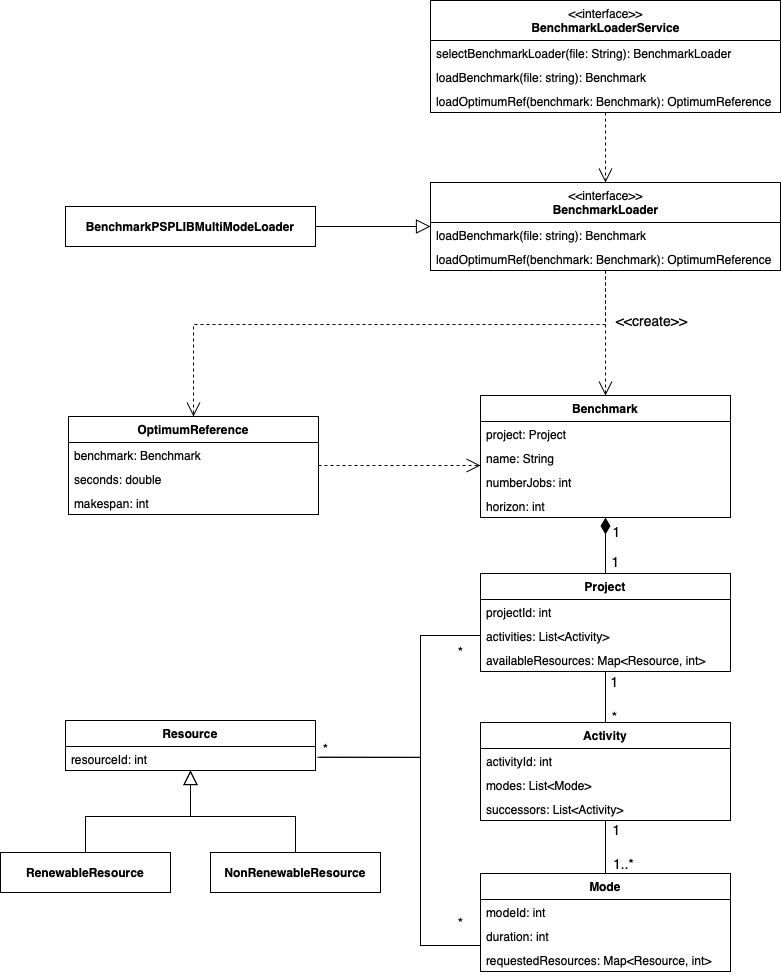
\includegraphics[width=0.85\textwidth]{assets/img/04_Umsetzung/BenchmarkLoaderInstanceSets.png}
    \caption{UML-Klassendiagramm für den Benchmark Loader} 
    \label{img:mrcpsp_framework_benchmarkloader}
    \source{Eigene Darstellung}
\end{figure}


\begin{figure}
    \centering
    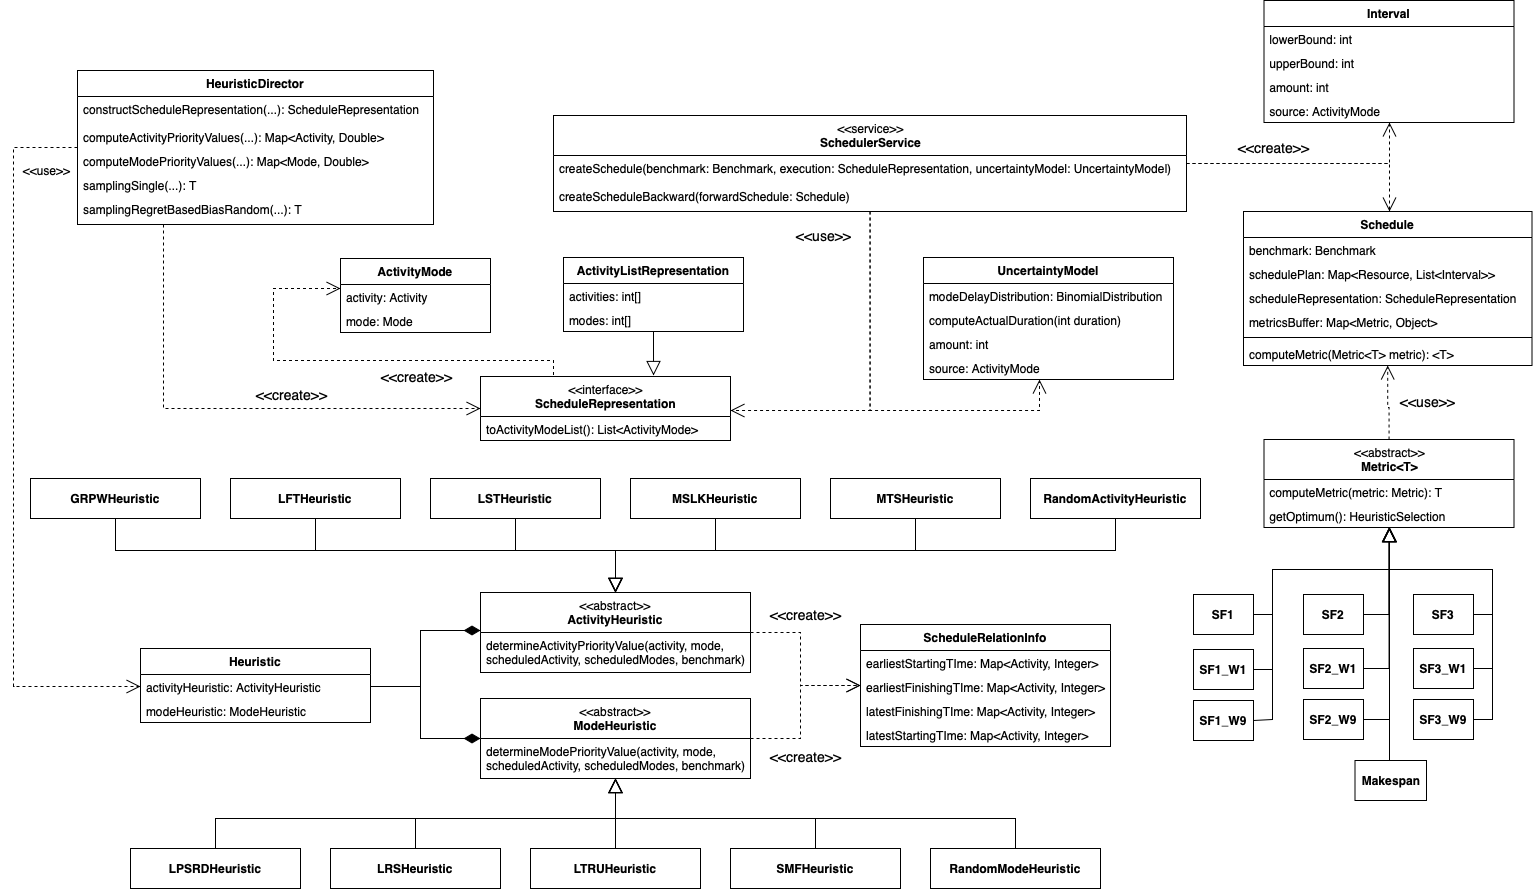
\includegraphics[angle=90,height=0.90\textheight]{assets/img/04_Umsetzung/Klassendiagramm_SchedulerHeuristiken.png}
    \caption{UML-Klassendiagramm für den Scheduler und Heuristiken} 
    \label{img:mrcpsp_framework_schedulerheuristiken}
    \source{Eigene Darstellung}
\end{figure}

\begin{figure}
    \centering
    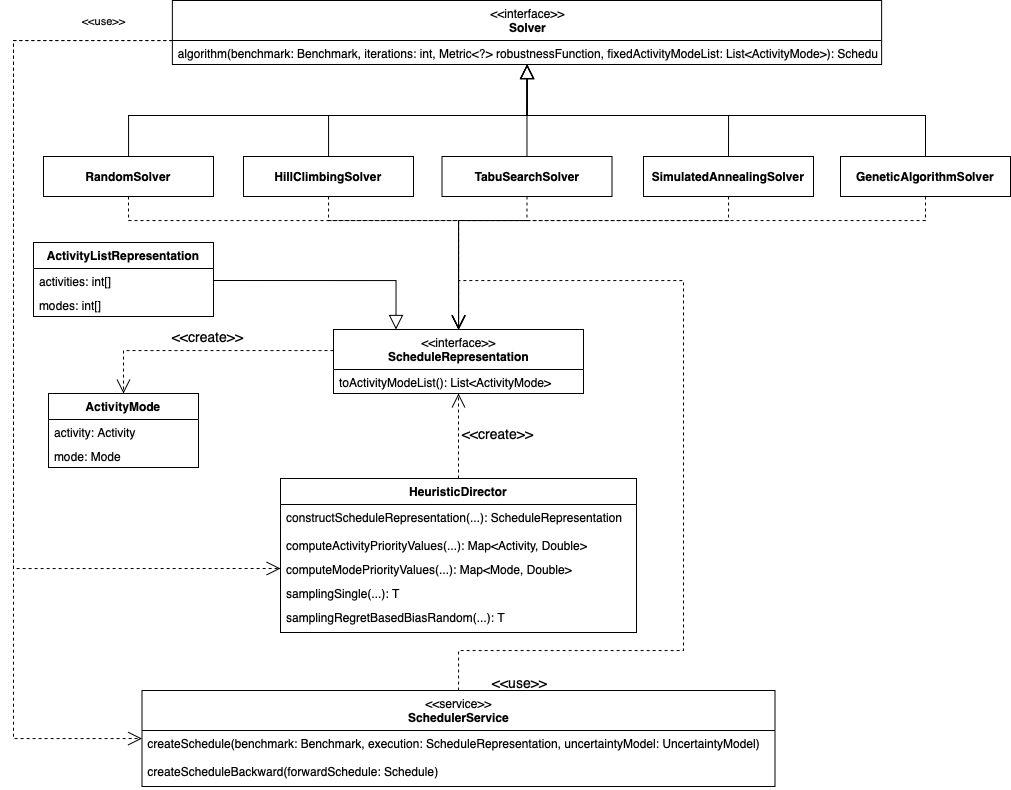
\includegraphics[width=1.06\textwidth]{assets/img/04_Umsetzung/KlassendiagrammSolver.png}
    \caption{UML-Klassendiagramm für die Solver} 
    \label{img:mrcpsp_framework_solver}
    \source{Eigene Darstellung}
\end{figure}

\begin{figure}
    \centering
    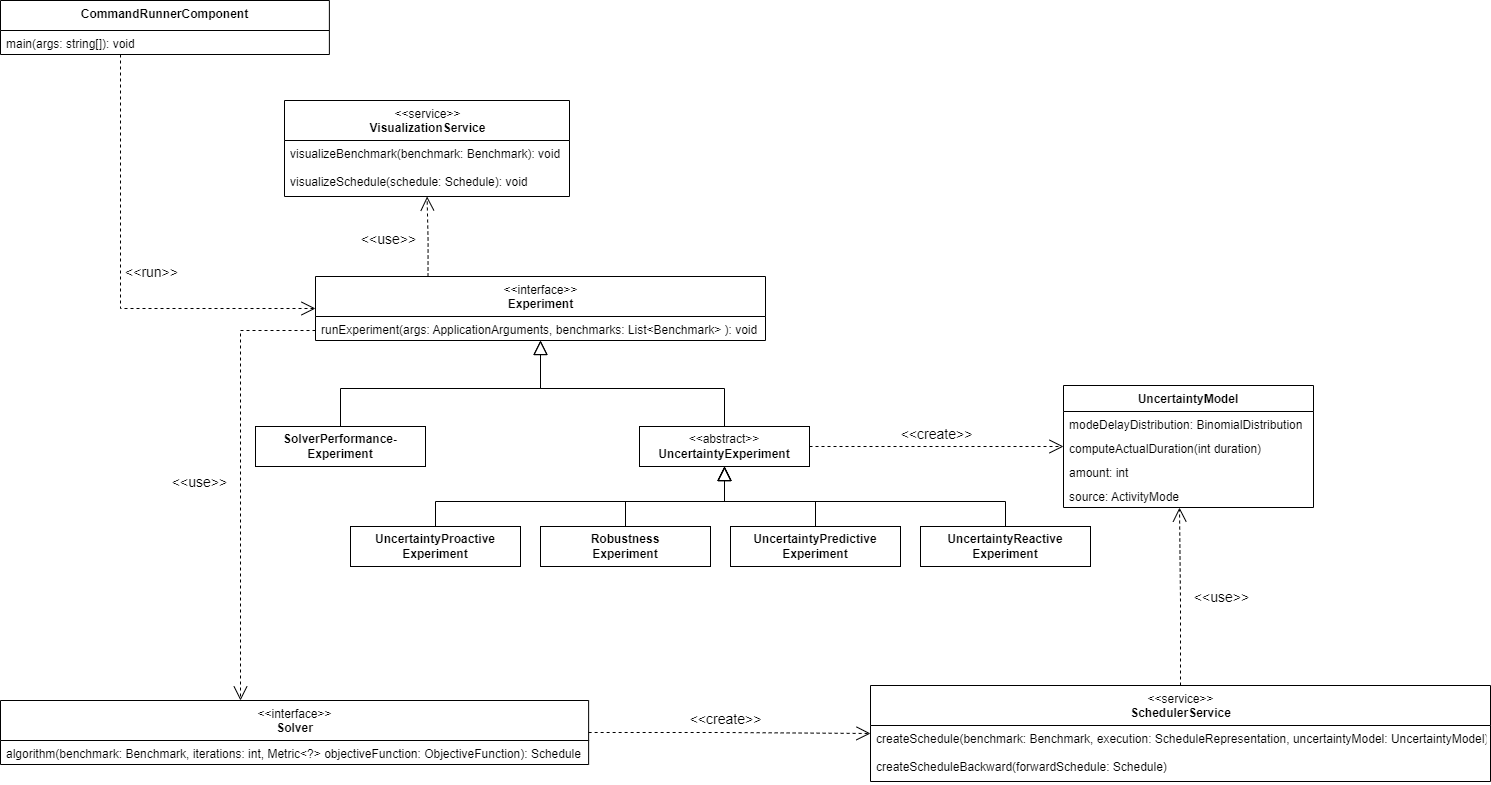
\includegraphics[angle=90,height=0.92\textheight]{assets/img/04_Umsetzung/Klassendiagramm_Experiments.drawio.png}
    \caption{UML-Klassendiagramm für die Experimente} 
    \label{img:mrcpsp_framework_experimente}
    \source{Eigene Darstellung}
\end{figure}

\chapter{Quellcode}

\begin{lstlisting}[caption={Erzeugen von Zeitplänen anhand von Aktivitäts- und Moduslisten}, label=lst:scheduler_forward, mathescape=truexinputencoding={utf8}, extendedchars=false, escapeinside=``, basicstyle=\scriptsize]
for (ActivityMode activityMode : activityModeList) {
  Mode currentMode = activityMode.getMode();
  // Create initial interval
  int potentialLowerBound = earliestStartTime.getOrDefault(activityMode.getActivity(), 0);

  // Construct the solution according the execution
  boolean solutionFound = false;
  while (!solutionFound) {
    solutionFound = true;
    for (Map.Entry<Resource, Integer> entry : currentMode.getRequestedResources().entrySet()) {
      Resource currentModeResource = entry.getKey();
      Integer currentModeAmount = entry.getValue();
      
      int resourceAvailableGeneral = benchmark.getProject().getAvailableResources()
                                .get(currentModeResource);
      int resourceAvailableOnInterval;
      
      if (currentModeResource instanceof RenewableResource) {
        int potentialUpperBound = potentialLowerBound + modeDurations.get(activityMode) - 1;

        // potential new interval that needs to be checked
        Interval potentialInterval = new Interval(potentialLowerBound,
                 potentialUpperBound,
                 currentModeAmount,
                 activityMode);

        resourceAvailableOnInterval = this.computeAvailableResourcesOnInterval(schedulePlan,
            currentModeResource, 
            potentialInterval, 
            resourceAvailableGeneral);
      } else {
        resourceAvailableOnInterval = nonRenewableResourcesLeft.get(currentModeResource);
      }

      if (currentModeAmount > resourceAvailableGeneral) {
        throw new RenewableResourceNotEnoughException();
      } else if (currentModeAmount > resourceAvailableOnInterval &&
              currentModeResource instanceof NonRenewableResource) {
            throw new NoNonRenewableResourcesLeftException(activityMode.getActivity());
      } else if (resourceAvailableOnInterval - currentModeAmount < 0) {
        solutionFound = false;
        potentialLowerBound++;
        break;
      }
    }
  }
  
  this.addInterval(activityMode,
    modeDurations.get(activityMode), 
    schedulePlan, 
    nonRenewableResourcesLeft, 
    earliestStartTime, 
    potentialLowerBound);
}
\end{lstlisting}

\begin{lstlisting}[caption={Algorithmus zur Berechnung von vorhandenen Ressourcen einer Ressourcenart für potentielles Intervall},label=lst:scheduler_computeAvailableResourcesOnInterval, mathescape=truexinputencoding={utf8}, extendedchars=false, escapeinside=``, basicstyle=\scriptsize]
private int computeAvailableResourcesOnInterval(Map<Resource, List<Interval>> scheduledPlan,
                                                Resource currentModeResource,
                                                Interval potentialInterval,
                                                int resourceAvailableGeneral) {
  int resourceAvailableOnInterval = resourceAvailableGeneral;
  List<Interval> conflictingIntervals = new ArrayList<>();

  // determine the actual resource availability on the given interval
  for (Interval intervalToCheck : scheduledPlan.get(currentModeResource)) {
    if (potentialInterval.conflictInterval(intervalToCheck)) {
      conflictingIntervals.add(intervalToCheck);
    }
  }

  // Calculate highest available resource at every timepoint
  for (int i = potentialInterval.getLowerBound(); i <= potentialInterval.getUpperBound(); i++) {
    int finalI = i;
    List<Interval> conflictingIntervalAtTimeslot = conflictingIntervals.stream()
            .filter(interval -> interval.valueInInterval(finalI)).collect(Collectors.toList());
    int availableAtTimeslot = resourceAvailableGeneral - conflictingIntervalAtTimeslot.stream()
            .map(Interval::getAmount).reduce((Integer::sum)).orElse(0);
    resourceAvailableOnInterval = Math.min(resourceAvailableOnInterval, availableAtTimeslot);
  }

  return resourceAvailableOnInterval;
}
\end{lstlisting}

\chapter{Auswertungen}
\label{ch:Auswertungen}

\section{Weitere Auswertung der implementierten Metaheuristiken}
\label{sec:WeitereAuswertung_Metaheuristiken}

\begin{table}[H]
\centering
\resizebox{\textwidth}{!}\\
Solver & Iteration &          &  &  & \\
\midrule
RandomSolver & 500  &     0.06 & 0.29 &      21.87 & 6.61 &   100.00 &   98.90 \\
                 & 1000 &     0.03 & 0.20 &      22.04 & 6.59 &   100.00 &   99.69 \\
                 & 2500 &     0.01 & 0.11 &      22.19 & 6.57 &   100.00 &  100.00 \\
                 & 5000 &     0.00 & 0.07 &      22.33 & 6.53 &   100.00 &   99.84 \\ \hline
HillClimbing & 500  &     1.83 & 2.96 &      21.11 & 6.34 &   100.00 &   63.27 \\
                 & 1000 &     1.85 & 2.98 &      21.16 & 6.38 &   100.00 &   63.42 \\
                 & 2500 &     1.85 & 2.99 &      21.09 & 6.39 &   100.00 &   62.64 \\
                 & 5000 &     1.85 & 2.97 &      21.17 & 6.39 &   100.00 &   62.32 \\ \hline
TabuSearch & 500  &     1.37 & 2.50 &      21.33 & 6.42 &   100.00 &   69.70 \\
                 & 1000 &     1.39 & 2.48 &      21.33 & 6.38 &   100.00 &   69.39 \\
                 & 2500 &     1.37 & 2.48 &      21.36 & 6.39 &   100.00 &   70.33 \\
                 & 5000 &     1.38 & 2.50 &      21.35 & 6.43 &   100.00 &   69.70 \\ \hline
SimulatedAnnealing & 500  &     1.31 & 2.43 &      21.53 & 6.30 &   100.00 &   76.77 \\ 
                 & 1000 &     1.14 & 2.21 &      21.66 & 6.30 &   100.00 &   80.38 \\
                 & 2500 &     0.88 & 1.91 &      21.90 & 6.24 &   100.00 &   84.62 \\
                 & 5000 &     0.70 & 1.71 &      21.96 & 6.28 &   100.00 &   88.70 \\ \hline
GeneticAlgorithm & 500  &     0.16 & 0.67 &      22.10 & 6.43 &   100.00 &   97.80 \\
                 & 1000 &     0.14 & 0.63 &      22.09 & 6.44 &   100.00 &   98.59 \\
                 & 2500 &     0.13 & 0.61 &      22.16 & 6.38 &   100.00 &   98.43 \\
                 & 5000 &     0.14 & 0.65 &      22.23 & 6.41 &   100.00 &   98.27 \\
\bottomrule
\end{tabular}
}
\caption{Vergleich der Lösungsverfahren für das Instanzset m1}
\source{Eigene Darstellung}
\label{tab:evaluation_solver_m1}
\end{table}


\begin{table}[H]
\centering
\resizebox{\textwidth}{!}\\
Solver & Iteration &          &  &  & \\
\midrule
RandomSolver & 500  &     2.76 & 3.43 &      17.57 & 5.87 &    99.79 &   41.04 \\
                 & 1000 &     2.26 & 3.11 &      18.23 & 5.68 &   100.00 &   47.50 \\
                 & 2500 &     1.62 & 2.59 &      18.26 & 5.97 &   100.00 &   59.38 \\
                 & 5000 &     1.30 & 2.17 &      18.45 & 6.27 &   100.00 &   63.96 \\ \hline
HillClimbing & 500  &     2.29 & 2.68 &      20.13 & 6.09 &   100.00 &   56.67 \\
                 & 1000 &     2.29 & 2.79 &      19.97 & 6.25 &   100.00 &   57.92 \\
                 & 2500 &     2.29 & 2.77 &      20.03 & 6.20 &   100.00 &   57.71 \\
                 & 5000 &     2.24 & 2.71 &      20.09 & 6.09 &   100.00 &   59.38 \\ \hline
TabuSearch & 500  &     1.65 & 2.27 &      20.39 & 6.34 &   100.00 &   70.42 \\
                 & 1000 &     1.35 & 2.03 &      20.21 & 6.28 &   100.00 &   78.12 \\
                 & 2500 &     1.05 & 1.80 &      20.20 & 6.39 &   100.00 &   86.04 \\
                 & 5000 &     0.86 & 1.71 &      20.21 & 6.42 &   100.00 &   89.38 \\ \hline
SimulatedAnnealing & 500  &     2.02 & 2.61 &      20.10 & 6.39 &   100.00 &   64.17 \\
                 & 1000 &     1.42 & 2.03 &      20.03 & 6.48 &   100.00 &   73.96 \\
                 & 2500 &     0.87 & 1.53 &      19.96 & 6.52 &   100.00 &   85.62 \\
                 & 5000 &     0.60 & 1.23 &      20.01 & 6.63 &   100.00 &   92.08 \\ \hline
GeneticAlgorithm & 500  &     1.36 & 1.74 &      19.52 & 6.50 &   100.00 &   61.25 \\
                 & 1000 &     0.64 & 1.09 &      19.62 & 6.57 &   100.00 &   82.71 \\
                 & 2500 &     0.40 & 0.84 &      19.87 & 6.48 &   100.00 &   89.17 \\
                 & 5000 &     0.33 & 0.75 &      19.76 & 6.52 &   100.00 &   92.50 \\
\bottomrule
\end{tabular}
}
\caption{Vergleich der Lösungsverfahren für das Instanzset m2}
\source{Eigene Darstellung}
\label{tab:evaluation_solver_m2}
\end{table}


\begin{table}[H]
\centering
\resizebox{\textwidth}{!}\\
Solver & Iteration &          &  &  & \\
\midrule
RandomSolver & 500  &     4.64 & 3.38 &      11.42 & 4.43 &   100.00 &   20.68 \\
                 & 1000 &     3.95 & 3.14 &      11.49 & 4.40 &   100.00 &   26.44 \\
                 & 2500 &     3.17 & 2.83 &      11.78 & 5.21 &   100.00 &   33.48 \\
                 & 5000 &     2.73 & 2.69 &      12.18 & 5.28 &   100.00 &   42.22 \\ \hline
HillClimbing & 500  &     1.30 & 2.16 &      15.94 & 6.66 &   100.00 &   78.46 \\
                 & 1000 &     1.17 & 2.01 &      16.25 & 6.91 &   100.00 &   78.46 \\
                 & 2500 &     1.09 & 1.94 &      16.02 & 6.81 &   100.00 &   80.60 \\
                 & 5000 &     1.10 & 1.96 &      16.13 & 6.81 &   100.00 &   80.60 \\  \hline
TabuSearch & 500  &     0.82 & 1.65 &      15.96 & 7.22 &   100.00 &   83.58 \\
                 & 1000 &     0.56 & 1.30 &      16.29 & 7.26 &   100.00 &   87.63 \\
                 & 2500 &     0.30 & 0.85 &      16.44 & 7.34 &   100.00 &   92.96 \\
                 & 5000 &     0.19 & 0.62 &      16.53 & 7.37 &   100.00 &   95.74 \\  \hline
SimulatedAnnealing & 500  &     1.60 & 2.25 &      15.45 & 6.80 &   100.00 &   72.71 \\
                 & 1000 &     0.83 & 1.50 &      16.01 & 7.21 &   100.00 &   80.38 \\
                 & 2500 &     0.40 & 0.90 &      16.29 & 7.54 &   100.00 &   89.77 \\
                 & 5000 &     0.23 & 0.59 &      16.34 & 7.61 &   100.00 &   92.32 \\ \hline
GeneticAlgorithm & 500  &     0.60 & 1.18 &      15.84 & 6.75 &   100.00 &   80.38 \\
                 & 1000 &     0.36 & 0.83 &      16.17 & 7.13 &   100.00 &   87.21 \\
                 & 2500 &     0.23 & 0.59 &      16.41 & 7.43 &   100.00 &   93.18 \\
                 & 5000 &     0.21 & 0.58 &      16.47 & 7.46 &   100.00 &   93.18 \\
\bottomrule
\end{tabular}
}
\caption{Vergleich der Lösungsverfahren für das Instanzset n0}
\source{Eigene Darstellung}
\label{tab:evaluation_solver_n0}
\end{table}


\begin{table}[H]
\centering
\resizebox{\textwidth}{!}\\
Solver & Iteration &          &  &  & \\
\midrule
RandomSolver & 500  &     7.18 & 9.29 &      16.19 & 4.52 &    99.28 &    2.35 \\
                 & 1000 &     7.05 & 7.17 &      18.62 & 5.42 &    99.28 &    3.25 \\
                 & 2500 &     6.25 & 5.70 &      17.94 & 5.00 &    99.28 &    6.14 \\
                 & 5000 &     5.56 & 5.39 &      18.73 & 4.86 &    99.28 &    7.40 \\ \hline
HillClimbing & 500  &     3.32 & 3.57 &      22.05 & 6.19 &   100.00 &   43.50 \\
                 & 1000 &     3.14 & 3.43 &      22.18 & 6.17 &   100.00 &   42.06 \\
                 & 2500 &     3.10 & 3.37 &      21.77 & 6.21 &   100.00 &   45.49 \\
                 & 5000 &     3.08 & 3.41 &      21.96 & 6.23 &   100.00 &   45.49 \\ \hline
TabuSearch & 500  &     2.75 & 3.13 &      22.12 & 6.57 &   100.00 &   48.92 \\
                 & 1000 &     2.26 & 2.81 &      22.20 & 6.80 &   100.00 &   55.23 \\
                 & 2500 &     1.76 & 2.46 &      22.20 & 6.86 &   100.00 &   62.82 \\
                 & 5000 &     1.40 & 2.08 &      22.12 & 7.12 &   100.00 &   70.22 \\ \hline
SimulatedAnnealing & 500  &     3.67 & 3.60 &      21.63 & 6.18 &   100.00 &   39.71 \\
                 & 1000 &     2.65 & 2.97 &      22.00 & 6.75 &   100.00 &   48.92 \\
                 & 2500 &     1.71 & 2.17 &      22.15 & 7.21 &   100.00 &   59.57 \\
                 & 5000 &     1.19 & 1.70 &      21.70 & 7.49 &   100.00 &   69.86 \\ \hline
GeneticAlgorithm & 500  &     3.43 & 3.69 &      21.25 & 6.05 &   100.00 &   38.81 \\
                 & 1000 &     1.92 & 2.21 &      21.75 & 6.78 &   100.00 &   49.10 \\
                 & 2500 &     0.97 & 1.30 &      21.53 & 7.36 &   100.00 &   66.25 \\
                 & 5000 &     0.72 & 1.09 &      21.38 & 7.48 &   100.00 &   75.99 \\
\bottomrule
\end{tabular}
}
\caption{Vergleich der Lösungsverfahren für das Instanzset j20}
\source{Eigene Darstellung}
\label{tab:evaluation_solver_j20}
\end{table}

\newpage

\section{Weitere Auswertung der proaktiven Verfahren}
\label{sec:WeitereAuswertung_Proaktiv}

{\footnotesize
\begin{longtable}{ll|rrrr|rrrr}
\toprule
\textbf{Instance set m1}                 & {} & \multicolumn{4}{c|}{Mean $\mu$} & \multicolumn{4}{c}{Std. Dev $\sigma$} \\
                & Uncertainty $p$: & 0\% & 5\% & 10\% & 20\% & 0\% & 5\% & 10\% & 20\% \\
Solver & Iteration &      &      &      &      &      &      &      &      \\
\midrule
RandomSolver & 500  & 0.05 & 0.93 & 1.75 & 3.26 & 0.24 & 1.33 & 1.76 & 2.20 \\
                 & 1000 & 0.05 & 0.91 & 1.71 & 3.20 & 0.25 & 1.31 & 1.69 & 2.15 \\
                 & 2500 & 0.03 & 0.92 & 1.73 & 3.26 & 0.16 & 1.42 & 1.80 & 2.25 \\
                 & 5000 & 0.02 & 0.92 & 1.72 & 3.22 & 0.14 & 1.35 & 1.75 & 2.21 \\ \hline
HillClimbing & 500  & 1.78 & 2.56 & 3.33 & 4.78 & 2.46 & 2.73 & 2.96 & 3.28 \\
                 & 1000 & 1.85 & 2.65 & 3.39 & 4.84 & 2.58 & 2.82 & 3.05 & 3.40 \\
                 & 2500 & 1.80 & 2.60 & 3.36 & 4.83 & 2.53 & 2.80 & 3.01 & 3.38 \\
                 & 5000 & 1.84 & 2.62 & 3.38 & 4.85 & 2.56 & 2.81 & 3.00 & 3.37 \\ \hline
TabuSearch & 500  & 1.40 & 2.21 & 2.99 & 4.47 & 2.12 & 2.43 & 2.69 & 3.06 \\
                 & 1000 & 1.34 & 2.17 & 2.94 & 4.42 & 2.07 & 2.42 & 2.67 & 3.04 \\
                 & 2500 & 1.33 & 2.16 & 2.93 & 4.44 & 2.04 & 2.40 & 2.64 & 3.06 \\
                 & 5000 & 1.37 & 2.20 & 2.97 & 4.46 & 2.16 & 2.51 & 2.74 & 3.13 \\ \hline
SimulatedAnnealing & 500  & 1.44 & 2.27 & 3.04 & 4.48 & 2.34 & 2.65 & 2.84 & 3.17 \\
                 & 1000 & 1.24 & 2.03 & 2.78 & 4.24 & 2.06 & 2.35 & 2.56 & 2.89 \\
                 & 2500 & 0.92 & 1.73 & 2.48 & 3.93 & 1.84 & 2.17 & 2.40 & 2.76 \\
                 & 5000 & 0.72 & 1.55 & 2.32 & 3.78 & 1.65 & 2.01 & 2.27 & 2.63 \\ \hline
GeneticAlgorithm & 500  & 0.14 & 1.05 & 1.84 & 3.34 & 0.59 & 1.56 & 1.94 & 2.43 \\
                 & 1000 & 0.08 & 1.01 & 1.85 & 3.36 & 0.36 & 1.61 & 2.08 & 2.58 \\
                 & 2500 & 0.09 & 1.02 & 1.84 & 3.38 & 0.43 & 1.70 & 2.13 & 2.64 \\
                 & 5000 & 0.09 & 0.97 & 1.79 & 3.31 & 0.41 & 1.45 & 1.87 & 2.38 \\
\bottomrule
\caption{Vergleich der proaktiven Lösungsverfahren auf $m=50$ unterschiedliche Unsicherheitsszenarien für das Instanzset m1. }
\label{tab:evaluation_proactive_m1}
\end{longtable}
}
\vspace*{-25px}
\begin{figure}[H]
\source{Eigene Darstellung}
\end{figure}

{\footnotesize
\begin{longtable}{ll|rrrr|rrrr}
\toprule
\textbf{Instance set m2}                 & {} & \multicolumn{4}{c|}{Mean $\mu$} & \multicolumn{4}{c}{Std. Dev $\sigma$} \\
                & Uncertainty $p$: & 0\% & 5\% & 10\% & 20\% & 0\% & 5\% & 10\% & 20\% \\
Solver & Iteration &      &      &      &      &      &      &      &      \\
\midrule
RandomSolver & 500  & 2.96 & 3.83 & 4.61 & 6.11 & 3.17 & 3.55 & 3.80 & 4.18 \\
                 & 1000 & 2.32 & 3.21 & 4.05 & 5.58 & 2.67 & 3.10 & 3.39 & 3.78 \\
                 & 2500 & 1.65 & 2.57 & 3.40 & 4.92 & 2.29 & 2.79 & 3.04 & 3.44 \\
                 & 5000 & 1.29 & 2.21 & 3.03 & 4.57 & 1.86 & 2.42 & 2.77 & 3.20 \\ \hline
HillClimbing & 500  & 2.93 & 3.78 & 4.58 & 6.00 & 3.45 & 3.71 & 3.91 & 4.15 \\
                 & 1000 & 3.04 & 3.90 & 4.67 & 6.10 & 3.50 & 3.78 & 3.95 & 4.20 \\
                 & 2500 & 2.90 & 3.77 & 4.56 & 5.99 & 3.54 & 3.83 & 4.05 & 4.31 \\
                 & 5000 & 2.87 & 3.78 & 4.58 & 6.04 & 3.40 & 3.80 & 4.02 & 4.24 \\ \hline
TabuSearch & 500  & 1.37 & 2.25 & 3.02 & 4.49 & 1.90 & 2.31 & 2.57 & 2.88 \\
                 & 1000 & 1.13 & 1.99 & 2.79 & 4.26 & 1.90 & 2.22 & 2.42 & 2.75 \\
                 & 2500 & 0.77 & 1.65 & 2.46 & 3.93 & 1.45 & 1.88 & 2.17 & 2.51 \\
                 & 5000 & 0.67 & 1.55 & 2.35 & 3.83 & 1.38 & 1.78 & 2.04 & 2.35 \\ \hline
SimulatedAnnealing & 500  & 1.89 & 2.74 & 3.50 & 4.99 & 2.31 & 2.60 & 2.80 & 3.11 \\
                 & 1000 & 1.19 & 2.08 & 2.90 & 4.35 & 1.75 & 2.17 & 2.45 & 2.73 \\
                 & 2500 & 0.74 & 1.60 & 2.38 & 3.83 & 1.25 & 1.70 & 1.93 & 2.30 \\
                 & 5000 & 0.50 & 1.41 & 2.24 & 3.67 & 1.04 & 1.73 & 2.18 & 2.48 \\ \hline
GeneticAlgorithm & 500  & 1.40 & 2.22 & 2.99 & 4.46 & 1.89 & 2.28 & 2.54 & 2.95 \\
                 & 1000 & 0.63 & 1.46 & 2.24 & 3.70 & 1.11 & 1.67 & 2.02 & 2.42 \\
                 & 2500 & 0.36 & 1.19 & 1.98 & 3.45 & 0.74 & 1.40 & 1.76 & 2.16 \\
                 & 5000 & 0.26 & 1.10 & 1.90 & 3.34 & 0.64 & 1.33 & 1.74 & 2.14 \\
\bottomrule
\caption{Vergleich der proaktiven Lösungsverfahren auf $m=50$ unterschiedliche Unsicherheitsszenarien für das Instanzset m2. }
\label{tab:evaluation_proactive_m2}
\end{longtable}
}
\vspace*{-25px}
\begin{figure}[H]
\source{Eigene Darstellung}
\end{figure}


{\footnotesize
\begin{longtable}{ll|rrrr|rrrr}
\toprule
\textbf{Instance set n0}                 & {} & \multicolumn{4}{c|}{Mean $\mu$} & \multicolumn{4}{c}{Std. Dev $\sigma$} \\
                & Uncertainty $p$: & 0\% & 5\% & 10\% & 20\% & 0\% & 5\% & 10\% & 20\% \\
Solver & Iteration &      &      &      &      &      &      &      &      \\
\midrule
RandomSolver & 500  & 4.48 & 5.30 & 6.06 & 7.51 & 3.24 & 3.58 & 3.85 & 4.29 \\
                 & 1000 & 3.82 & 4.63 & 5.40 & 6.78 & 3.07 & 3.48 & 3.80 & 4.17 \\
                 & 2500 & 3.09 & 3.95 & 4.71 & 6.15 & 2.81 & 3.29 & 3.55 & 4.08 \\
                 & 5000 & 2.62 & 3.46 & 4.22 & 5.67 & 2.62 & 2.97 & 3.26 & 3.73 \\ \hline
HillClimbing & 500  & 3.19 & 4.15 & 4.97 & 6.44 & 3.69 & 4.13 & 4.44 & 4.85 \\
                 & 1000 & 3.21 & 4.21 & 5.07 & 6.52 & 3.90 & 4.44 & 4.81 & 5.20 \\
                 & 2500 & 3.31 & 4.28 & 5.11 & 6.69 & 3.84 & 4.38 & 4.63 & 5.14 \\
                 & 5000 & 3.11 & 4.10 & 4.94 & 6.47 & 3.69 & 4.20 & 4.55 & 5.05 \\ \hline
TabuSearch & 500  & 1.01 & 1.94 & 2.71 & 4.22 & 1.85 & 2.48 & 2.80 & 3.38 \\
                 & 1000 & 0.57 & 1.47 & 2.26 & 3.70 & 1.32 & 1.95 & 2.31 & 2.80 \\
                 & 2500 & 0.24 & 1.17 & 1.97 & 3.44 & 0.73 & 1.74 & 2.13 & 2.61 \\
                 & 5000 & 0.12 & 1.07 & 1.88 & 3.33 & 0.45 & 1.54 & 1.93 & 2.38 \\ \hline
SimulatedAnnealing & 500  & 1.97 & 2.88 & 3.67 & 5.13 & 2.60 & 3.08 & 3.40 & 3.80 \\
                 & 1000 & 1.05 & 1.97 & 2.77 & 4.21 & 1.81 & 2.33 & 2.67 & 3.05 \\
                 & 2500 & 0.42 & 1.32 & 2.11 & 3.57 & 1.12 & 1.72 & 2.04 & 2.56 \\
                 & 5000 & 0.24 & 1.17 & 1.98 & 3.48 & 0.70 & 1.47 & 1.85 & 2.31 \\ \hline
GeneticAlgorithm & 500  & 0.57 & 1.38 & 2.14 & 3.54 & 1.19 & 1.72 & 2.07 & 2.54 \\
                 & 1000 & 0.26 & 1.09 & 1.83 & 3.28 & 0.67 & 1.39 & 1.74 & 2.25 \\
                 & 2500 & 0.16 & 0.99 & 1.75 & 3.18 & 0.46 & 1.25 & 1.66 & 2.17 \\
                 & 5000 & 0.13 & 0.97 & 1.70 & 3.15 & 0.44 & 1.24 & 1.58 & 2.10 \\
\bottomrule
\caption{Vergleich der proaktiven Lösungsverfahren auf $m=50$ unterschiedliche Unsicherheitsszenarien für das Instanzset n0. }
\label{tab:evaluation_proactive_n0}
\end{longtable}
}
\vspace*{-25px}
\begin{figure}[H]
\source{Eigene Darstellung}
\end{figure}

\newpage

\section{Weitere Auswertung der prädiktiven Verfahren}
\label{sec:WeitereAuswertung_Prädiktiv}

\subsection{Vergleich der unterschiedlichen Robustheitsmessungen}
\label{sec:WeitereAuswertung_Robustness}

{\fontsize{9.5}{10.5} \selectfont
\begin{longtable}{ll|rrrr|rrrr}
\toprule
\textbf{Instance set n1}                 & {} & \multicolumn{4}{c|}{Mean $\mu$} & \multicolumn{4}{c}{Std. Dev $\sigma$} \\
\textbf{RandomSolver}                 & Uncertainty $p$: & 0\% & 5\% & 10\% & 20\% & 0\% & 5\% & 10\% & 20\% \\
Iteration & $\Omega(x)$ &      &      &      &      &      &      &      &      \\
\midrule
500  & No-RM & 0.00 & 0.82 & 1.62 & 3.09 & 0.00 & 1.16 & 1.62 & 2.07 \\
     & SF1 & 0.00 & 0.85 & 1.65 & 3.12 & 0.00 & 1.26 & 1.72 & 2.23 \\
     & SF1\_W1 & 0.00 & 0.83 & 1.61 & 3.06 & 0.00 & 1.24 & 1.65 & 2.11 \\
     & SF1\_W9 & 0.00 & 0.83 & 1.61 & 3.11 & 0.00 & 1.18 & 1.58 & 2.05 \\
     & SF2 & 0.00 & 0.83 & 1.59 & 3.03 & 0.00 & 1.22 & 1.59 & 2.06 \\
     & SF2\_W1 & 0.00 & 0.82 & 1.56 & 3.05 & 0.00 & 1.27 & 1.65 & 2.12 \\
     & SF2\_W9 & 0.00 & 0.84 & 1.62 & 3.08 & 0.00 & 1.32 & 1.71 & 2.17 \\
     & SF3 & 0.00 & 0.85 & 1.63 & 3.15 & 0.00 & 1.31 & 1.71 & 2.22 \\
     & SF3\_W1 & 0.00 & 0.83 & 1.62 & 3.06 & 0.00 & 1.22 & 1.65 & 2.06 \\
     & SF3\_W9 & 0.00 & 0.80 & 1.58 & 3.04 & 0.00 & 1.07 & 1.46 & 1.90 \\ \hline
1000 & No-RM & 0.00 & 0.88 & 1.69 & 3.22 & 0.00 & 1.32 & 1.73 & 2.22 \\
     & SF1 & 0.00 & 0.81 & 1.60 & 3.09 & 0.00 & 1.18 & 1.63 & 2.13 \\
     & SF1\_W1 & 0.00 & 0.89 & 1.69 & 3.23 & 0.00 & 1.39 & 1.75 & 2.26 \\
     & SF1\_W9 & 0.00 & 0.85 & 1.65 & 3.13 & 0.00 & 1.29 & 1.70 & 2.18 \\
     & SF2 & 0.00 & 0.81 & 1.58 & 3.04 & 0.00 & 1.18 & 1.56 & 2.00 \\
     & SF2\_W1 & 0.00 & 0.79 & 1.54 & 3.02 & 0.00 & 1.06 & 1.45 & 1.95 \\
     & SF2\_W9 & 0.00 & 0.83 & 1.62 & 3.07 & 0.00 & 1.18 & 1.59 & 2.03 \\
     & SF3 & 0.00 & 0.82 & 1.56 & 3.04 & 0.00 & 1.17 & 1.48 & 2.02 \\
     & SF3\_W1 & 0.00 & 0.81 & 1.60 & 3.08 & 0.00 & 1.12 & 1.50 & 1.99 \\
     & SF3\_W9 & 0.00 & 0.81 & 1.61 & 3.08 & 0.00 & 1.16 & 1.60 & 2.06 \\ \hline
2500 & No-RM & 0.00 & 0.86 & 1.67 & 3.19 & 0.00 & 1.24 & 1.64 & 2.18 \\
     & SF1 & 0.00 & 0.82 & 1.61 & 3.07 & 0.00 & 1.19 & 1.57 & 1.98 \\
     & SF1\_W1 & 0.00 & 0.87 & 1.66 & 3.16 & 0.00 & 1.22 & 1.65 & 2.06 \\
     & SF1\_W9 & 0.00 & 0.86 & 1.65 & 3.14 & 0.00 & 1.28 & 1.65 & 2.12 \\
     & SF2 & 0.00 & 0.82 & 1.58 & 3.05 & 0.00 & 1.24 & 1.61 & 2.07 \\
     & SF2\_W1 & 0.00 & 0.81 & 1.59 & 3.09 & 0.00 & 1.14 & 1.55 & 2.02 \\
     & SF2\_W9 & 0.00 & 0.82 & 1.60 & 3.06 & 0.00 & 1.17 & 1.57 & 2.04 \\
     & SF3 & 0.00 & 0.83 & 1.62 & 3.07 & 0.00 & 1.16 & 1.53 & 1.96 \\
     & SF3\_W1 & 0.00 & 0.83 & 1.63 & 3.11 & 0.00 & 1.21 & 1.70 & 2.14 \\
     & SF3\_W9 & 0.00 & 0.87 & 1.67 & 3.16 & 0.00 & 1.19 & 1.58 & 2.02 \\ \hline
5000 & No-RM & 0.00 & 0.89 & 1.70 & 3.18 & 0.00 & 1.27 & 1.63 & 2.09 \\
     & SF1 & 0.00 & 0.86 & 1.67 & 3.17 & 0.00 & 1.21 & 1.64 & 2.04 \\
     & SF1\_W1 & 0.00 & 0.86 & 1.65 & 3.15 & 0.00 & 1.25 & 1.66 & 2.11 \\
     & SF1\_W9 & 0.00 & 0.84 & 1.64 & 3.15 & 0.00 & 1.17 & 1.57 & 2.02 \\
     & SF2 & 0.00 & 0.83 & 1.62 & 3.11 & 0.00 & 1.23 & 1.60 & 2.12 \\
     & SF2\_W1 & 0.00 & 0.83 & 1.61 & 3.09 & 0.00 & 1.14 & 1.53 & 1.98 \\
     & SF2\_W9 & 0.00 & 0.87 & 1.68 & 3.20 & 0.00 & 1.24 & 1.63 & 2.14 \\
     & SF3 & 0.00 & 0.84 & 1.63 & 3.12 & 0.00 & 1.21 & 1.60 & 2.04 \\
     & SF3\_W1 & 0.00 & 0.84 & 1.64 & 3.15 & 0.00 & 1.17 & 1.60 & 2.04 \\
     & SF3\_W9 & 0.00 & 0.91 & 1.72 & 3.23 & 0.00 & 1.41 & 1.82 & 2.29 \\
\bottomrule
\caption{Verspätungswerte der Robustheitfunktionen $\Omega(x)$ angewendet auf den \acs{RS} für das Instanzset n1 mit $n = 50$ Unsicherheitsszenarien. }
\label{tab:evaluation_robustness_n1_ra}
\end{longtable}
}
\vspace*{-25px}
\begin{figure}[H]
\source{Eigene Darstellung}
\end{figure}

\newpage

{\fontsize{10}{11} \selectfont
\begin{longtable}{ll|rrrr|rrrr}
\toprule
\textbf{Instance set n1}                 & {} & \multicolumn{4}{c|}{Mean $\mu$} & \multicolumn{4}{c}{Std. Dev $\sigma$} \\
\textbf{HillClimbing}                 & Uncertainty $p$: & 0\% & 5\% & 10\% & 20\% & 0\% & 5\% & 10\% & 20\% \\
Iteration & $\Omega(x)$ &      &      &      &      &      &      &      &      \\
\midrule
500  & No-RM & 0.00 & 0.97 & 1.81 & 3.33 & 0.00 & 1.27 & 1.62 & 2.03 \\
     & SF1 & 0.00 & 0.92 & 1.72 & 3.26 & 0.00 & 1.41 & 1.78 & 2.28 \\
     & SF1\_W1 & 0.00 & 0.87 & 1.68 & 3.17 & 0.00 & 1.21 & 1.63 & 2.11 \\
     & SF1\_W9 & 0.00 & 0.93 & 1.75 & 3.28 & 0.00 & 1.35 & 1.75 & 2.25 \\
     & SF2 & 0.00 & 0.87 & 1.64 & 3.16 & 0.00 & 1.32 & 1.76 & 2.25 \\
     & SF2\_W1 & 0.00 & 0.85 & 1.61 & 3.13 & 0.00 & 1.26 & 1.66 & 2.17 \\
     & SF2\_W9 & 0.00 & 0.82 & 1.59 & 3.09 & 0.00 & 1.20 & 1.59 & 2.11 \\
     & SF3 & 0.00 & 0.91 & 1.75 & 3.30 & 0.00 & 1.43 & 1.86 & 2.39 \\
     & SF3\_W1 & 0.00 & 0.87 & 1.66 & 3.19 & 0.00 & 1.23 & 1.62 & 2.12 \\
     & SF3\_W9 & 0.00 & 0.89 & 1.68 & 3.21 & 0.00 & 1.28 & 1.65 & 2.20 \\ \hline
1000 & No-RM & 0.00 & 0.96 & 1.80 & 3.34 & 0.00 & 1.16 & 1.52 & 2.02 \\
     & SF1 & 0.00 & 0.94 & 1.78 & 3.31 & 0.00 & 1.39 & 1.79 & 2.29 \\
     & SF1\_W1 & 0.00 & 0.88 & 1.68 & 3.19 & 0.00 & 1.16 & 1.57 & 2.05 \\
     & SF1\_W9 & 0.00 & 0.90 & 1.71 & 3.22 & 0.00 & 1.32 & 1.72 & 2.23 \\
     & SF2 & 0.00 & 0.82 & 1.61 & 3.07 & 0.00 & 1.13 & 1.54 & 2.01 \\
     & SF2\_W1 & 0.00 & 0.83 & 1.59 & 3.13 & 0.00 & 1.16 & 1.52 & 2.10 \\
     & SF2\_W9 & 0.00 & 0.87 & 1.68 & 3.18 & 0.00 & 1.28 & 1.71 & 2.17 \\
     & SF3 & 0.00 & 0.87 & 1.69 & 3.19 & 0.00 & 1.22 & 1.65 & 2.09 \\
     & SF3\_W1 & 0.00 & 0.90 & 1.73 & 3.27 & 0.00 & 1.33 & 1.70 & 2.21 \\
     & SF3\_W9 & 0.00 & 0.89 & 1.72 & 3.24 & 0.00 & 1.30 & 1.70 & 2.18 \\ \hline
2500 & No-RM & 0.00 & 0.96 & 1.80 & 3.35 & 0.00 & 1.22 & 1.63 & 2.16 \\
     & SF1 & 0.00 & 0.95 & 1.75 & 3.29 & 0.00 & 1.43 & 1.79 & 2.28 \\
     & SF1\_W1 & 0.00 & 0.88 & 1.70 & 3.20 & 0.00 & 1.25 & 1.66 & 2.14 \\
     & SF1\_W9 & 0.00 & 0.93 & 1.75 & 3.25 & 0.00 & 1.33 & 1.71 & 2.20 \\
     & SF2 & 0.00 & 0.87 & 1.66 & 3.17 & 0.00 & 1.25 & 1.68 & 2.31 \\
     & SF2\_W1 & 0.00 & 0.85 & 1.62 & 3.13 & 0.00 & 1.25 & 1.61 & 2.13 \\
     & SF2\_W9 & 0.00 & 0.85 & 1.64 & 3.15 & 0.00 & 1.19 & 1.56 & 2.07 \\
     & SF3 & 0.00 & 0.91 & 1.72 & 3.25 & 0.00 & 1.33 & 1.72 & 2.21 \\
     & SF3\_W1 & 0.00 & 0.92 & 1.72 & 3.24 & 0.00 & 1.43 & 1.80 & 2.22 \\
     & SF3\_W9 & 0.00 & 0.87 & 1.69 & 3.19 & 0.00 & 1.28 & 1.64 & 2.11 \\ \hline
5000 & No-RM & 0.00 & 0.99 & 1.87 & 3.40 & 0.00 & 1.35 & 1.72 & 2.14 \\
     & SF1 & 0.00 & 0.88 & 1.68 & 3.17 & 0.00 & 1.21 & 1.59 & 2.08 \\
     & SF1\_W1 & 0.00 & 0.92 & 1.75 & 3.24 & 0.00 & 1.38 & 1.78 & 2.26 \\
     & SF1\_W9 & 0.00 & 0.88 & 1.70 & 3.19 & 0.00 & 1.20 & 1.59 & 2.08 \\
     & SF2 & 0.00 & 0.84 & 1.64 & 3.11 & 0.00 & 1.21 & 1.65 & 2.09 \\
     & SF2\_W1 & 0.00 & 0.83 & 1.61 & 3.09 & 0.00 & 1.24 & 1.59 & 2.05 \\
     & SF2\_W9 & 0.00 & 0.87 & 1.67 & 3.16 & 0.00 & 1.28 & 1.64 & 2.15 \\
     & SF3 & 0.00 & 0.90 & 1.70 & 3.24 & 0.00 & 1.30 & 1.68 & 2.20 \\
     & SF3\_W1 & 0.00 & 0.86 & 1.68 & 3.15 & 0.00 & 1.15 & 1.52 & 1.93 \\
     & SF3\_W9 & 0.00 & 0.89 & 1.71 & 3.22 & 0.00 & 1.37 & 1.73 & 2.24 \\
\bottomrule
\caption{Verspätungswerte der Robustheitfunktionen $\Omega(x)$ angewendet auf HC für das Instanzset n1 mit $n = 50$ Unsicherheitsszenarien. }
\label{tab:evaluation_robustness_n1_hc}
\end{longtable}
}
\vspace*{-25px}
\begin{figure}[H]
\source{Eigene Darstellung}
\end{figure}

\newpage

{\fontsize{10}{11} \selectfont
\begin{longtable}{ll|rrrr|rrrr}
\toprule
\textbf{Instance set n1}                 & {} & \multicolumn{4}{c|}{Mean $\mu$} & \multicolumn{4}{c}{Std. Dev $\sigma$} \\
\textbf{SimulatedAnnealing}                 & Uncertainty $p$: & 0\% & 5\% & 10\% & 20\% & 0\% & 5\% & 10\% & 20\% \\
Iteration & $\Omega(x)$ &      &      &      &      &      &      &      &      \\
\midrule
500  & No-RM & 0.00 & 0.93 & 1.74 & 3.28 & 0.00 & 1.25 & 1.63 & 2.12 \\
     & SF1 & 0.00 & 0.86 & 1.65 & 3.09 & 0.00 & 1.15 & 1.49 & 1.95 \\
     & SF1\_W1 & 0.00 & 0.86 & 1.66 & 3.14 & 0.00 & 1.21 & 1.56 & 2.04 \\
     & SF1\_W9 & 0.00 & 0.90 & 1.69 & 3.18 & 0.00 & 1.26 & 1.64 & 2.15 \\
     & SF2 & 0.00 & 0.82 & 1.61 & 3.09 & 0.00 & 1.16 & 1.58 & 2.06 \\
     & SF2\_W1 & 0.00 & 0.84 & 1.64 & 3.10 & 0.00 & 1.23 & 1.60 & 2.08 \\
     & SF2\_W9 & 0.00 & 0.86 & 1.66 & 3.14 & 0.00 & 1.29 & 1.69 & 2.17 \\
     & SF3 & 0.00 & 0.82 & 1.60 & 3.07 & 0.00 & 1.09 & 1.44 & 1.90 \\
     & SF3\_W1 & 0.00 & 0.85 & 1.66 & 3.14 & 0.00 & 1.17 & 1.56 & 2.07 \\
     & SF3\_W9 & 0.00 & 0.83 & 1.64 & 3.13 & 0.00 & 1.21 & 1.61 & 2.11 \\ \hline
1000 & No-RM & 0.00 & 0.98 & 1.80 & 3.34 & 0.00 & 1.20 & 1.55 & 1.98 \\
     & SF1 & 0.00 & 0.87 & 1.65 & 3.12 & 0.00 & 1.15 & 1.51 & 1.93 \\
     & SF1\_W1 & 0.00 & 0.89 & 1.66 & 3.15 & 0.00 & 1.26 & 1.61 & 2.10 \\
     & SF1\_W9 & 0.00 & 0.88 & 1.69 & 3.14 & 0.00 & 1.20 & 1.58 & 2.00 \\
     & SF2 & 0.00 & 0.85 & 1.62 & 3.10 & 0.00 & 1.21 & 1.58 & 2.06 \\
     & SF2\_W1 & 0.00 & 0.85 & 1.64 & 3.14 & 0.00 & 1.16 & 1.54 & 2.05 \\
     & SF2\_W9 & 0.00 & 0.91 & 1.72 & 3.25 & 0.00 & 1.40 & 1.77 & 2.27 \\
     & SF3 & 0.00 & 0.86 & 1.68 & 3.18 & 0.00 & 1.23 & 1.67 & 2.12 \\
     & SF3\_W1 & 0.00 & 0.87 & 1.67 & 3.16 & 0.00 & 1.11 & 1.52 & 1.92 \\
     & SF3\_W9 & 0.00 & 0.85 & 1.69 & 3.18 & 0.00 & 1.17 & 1.64 & 2.08 \\ \hline
2500 & No-RM & 0.00 & 0.97 & 1.82 & 3.34 & 0.00 & 1.24 & 1.59 & 2.01 \\
     & SF1 & 0.00 & 0.91 & 1.74 & 3.26 & 0.00 & 1.27 & 1.67 & 2.13 \\
     & SF1\_W1 & 0.00 & 0.91 & 1.74 & 3.23 & 0.00 & 1.27 & 1.66 & 2.10 \\
     & SF1\_W9 & 0.00 & 0.93 & 1.74 & 3.28 & 0.00 & 1.32 & 1.68 & 2.13 \\
     & SF2 & 0.00 & 0.83 & 1.61 & 3.10 & 0.00 & 1.10 & 1.48 & 1.90 \\
     & SF2\_W1 & 0.00 & 0.87 & 1.69 & 3.19 & 0.00 & 1.24 & 1.61 & 2.12 \\
     & SF2\_W9 & 0.00 & 0.88 & 1.66 & 3.20 & 0.00 & 1.25 & 1.59 & 2.11 \\
     & SF3 & 0.00 & 0.87 & 1.70 & 3.18 & 0.00 & 1.22 & 1.61 & 2.03 \\
     & SF3\_W1 & 0.00 & 0.89 & 1.70 & 3.21 & 0.00 & 1.22 & 1.61 & 2.07 \\
     & SF3\_W9 & 0.00 & 0.89 & 1.70 & 3.21 & 0.00 & 1.27 & 1.70 & 2.15 \\ \hline
5000 & No-RM & 0.00 & 0.97 & 1.81 & 3.33 & 0.00 & 1.15 & 1.53 & 1.93 \\
     & SF1 & 0.00 & 0.92 & 1.74 & 3.24 & 0.00 & 1.21 & 1.60 & 2.04 \\
     & SF1\_W1 & 0.00 & 0.89 & 1.69 & 3.16 & 0.00 & 1.22 & 1.56 & 2.01 \\
     & SF1\_W9 & 0.00 & 0.91 & 1.73 & 3.21 & 0.00 & 1.20 & 1.55 & 1.99 \\
     & SF2 & 0.00 & 0.84 & 1.64 & 3.16 & 0.00 & 1.11 & 1.48 & 1.93 \\
     & SF2\_W1 & 0.00 & 0.84 & 1.62 & 3.10 & 0.00 & 1.08 & 1.42 & 1.86 \\
     & SF2\_W9 & 0.00 & 0.85 & 1.66 & 3.17 & 0.00 & 1.18 & 1.56 & 2.04 \\
     & SF3 & 0.00 & 0.88 & 1.71 & 3.25 & 0.00 & 1.18 & 1.61 & 2.05 \\
     & SF3\_W1 & 0.00 & 0.87 & 1.69 & 3.19 & 0.00 & 1.20 & 1.63 & 2.07 \\
     & SF3\_W9 & 0.00 & 0.89 & 1.67 & 3.21 & 0.00 & 1.22 & 1.58 & 2.04 \\
\bottomrule
\caption{Verspätungswerte der Robustheitfunktionen $\Omega(x)$ angewendet auf \acs{SA} für das Instanzset n1 mit $n = 50$ Unsicherheitsszenarien. }
\label{tab:evaluation_robustness_n1_sa}
\end{longtable}
}
\vspace*{-25px}
\begin{figure}[H]
\source{Eigene Darstellung}
\end{figure}

\newpage

{\fontsize{10}{11} \selectfont
\begin{longtable}{ll|rrrr|rrrr}
\toprule
\textbf{Instance set n1}                 & {} & \multicolumn{4}{c|}{Mean $\mu$} & \multicolumn{4}{c}{Std. Dev $\sigma$} \\
\textbf{GeneticAlgorithm}                 & Uncertainty $p$: & 0\% & 5\% & 10\% & 20\% & 0\% & 5\% & 10\% & 20\% \\
Iteration & $\Omega(x)$ &      &      &      &      &      &      &      &      \\
\midrule
500  & No-RM & 0.00 & 0.86 & 1.66 & 3.18 & 0.00 & 1.06 & 1.40 & 1.90 \\
     & SF1 & 0.00 & 0.84 & 1.60 & 3.11 & 0.00 & 1.05 & 1.40 & 1.87 \\
     & SF1\_W1 & 0.00 & 0.83 & 1.61 & 3.08 & 0.00 & 1.08 & 1.45 & 1.86 \\
     & SF1\_W9 & 0.00 & 0.84 & 1.62 & 3.11 & 0.00 & 1.10 & 1.51 & 1.92 \\
     & SF2 & 0.00 & 0.85 & 1.65 & 3.16 & 0.00 & 1.16 & 1.56 & 2.02 \\
     & SF2\_W1 & 0.00 & 0.80 & 1.57 & 3.04 & 0.00 & 0.98 & 1.34 & 1.83 \\
     & SF2\_W9 & 0.00 & 0.81 & 1.59 & 3.05 & 0.00 & 1.06 & 1.42 & 1.82 \\
     & SF3 & 0.00 & 0.80 & 1.56 & 3.03 & 0.00 & 1.00 & 1.33 & 1.77 \\
     & SF3\_W1 & 0.00 & 0.81 & 1.58 & 3.06 & 0.00 & 1.01 & 1.41 & 1.82 \\
     & SF3\_W9 & 0.00 & 0.82 & 1.60 & 3.09 & 0.00 & 1.05 & 1.42 & 1.87 \\ \hline
1000 & No-RM & 0.00 & 0.92 & 1.75 & 3.24 & 0.00 & 1.18 & 1.59 & 1.98 \\
     & SF1 & 0.00 & 0.88 & 1.69 & 3.17 & 0.00 & 1.18 & 1.53 & 1.98 \\
     & SF1\_W1 & 0.00 & 0.86 & 1.64 & 3.13 & 0.00 & 1.05 & 1.39 & 1.81 \\
     & SF1\_W9 & 0.00 & 0.88 & 1.68 & 3.15 & 0.00 & 1.10 & 1.46 & 1.89 \\
     & SF2 & 0.00 & 0.84 & 1.61 & 3.07 & 0.00 & 1.07 & 1.40 & 1.80 \\
     & SF2\_W1 & 0.00 & 0.82 & 1.61 & 3.09 & 0.00 & 1.07 & 1.42 & 1.85 \\
     & SF2\_W9 & 0.00 & 0.85 & 1.64 & 3.12 & 0.00 & 1.09 & 1.45 & 1.85 \\
     & SF3 & 0.00 & 0.85 & 1.65 & 3.15 & 0.00 & 1.08 & 1.43 & 1.86 \\
     & SF3\_W1 & 0.00 & 0.86 & 1.66 & 3.15 & 0.00 & 1.12 & 1.47 & 1.93 \\
     & SF3\_W9 & 0.00 & 0.86 & 1.68 & 3.18 & 0.00 & 1.19 & 1.63 & 2.03 \\ \hline
2500 & No-RM & 0.00 & 0.91 & 1.72 & 3.23 & 0.00 & 1.06 & 1.41 & 1.82 \\
     & SF1 & 0.00 & 0.90 & 1.71 & 3.19 & 0.00 & 1.17 & 1.49 & 1.91 \\
     & SF1\_W1 & 0.00 & 0.89 & 1.70 & 3.20 & 0.00 & 1.15 & 1.49 & 1.96 \\
     & SF1\_W9 & 0.00 & 0.89 & 1.70 & 3.20 & 0.00 & 1.11 & 1.45 & 1.90 \\
     & SF2 & 0.00 & 0.82 & 1.61 & 3.06 & 0.00 & 1.07 & 1.42 & 1.81 \\
     & SF2\_W1 & 0.00 & 0.87 & 1.65 & 3.17 & 0.00 & 1.14 & 1.46 & 1.90 \\
     & SF2\_W9 & 0.00 & 0.86 & 1.66 & 3.14 & 0.00 & 1.09 & 1.47 & 1.91 \\
     & SF3 & 0.00 & 0.87 & 1.67 & 3.17 & 0.00 & 1.12 & 1.47 & 1.91 \\
     & SF3\_W1 & 0.00 & 0.83 & 1.63 & 3.07 & 0.00 & 1.01 & 1.35 & 1.72 \\
     & SF3\_W9 & 0.00 & 0.84 & 1.64 & 3.14 & 0.00 & 1.03 & 1.40 & 1.81 \\ \hline
5000 & No-RM & 0.00 & 0.94 & 1.78 & 3.29 & 0.00 & 1.18 & 1.54 & 1.90 \\
     & SF1 & 0.00 & 0.93 & 1.77 & 3.30 & 0.00 & 1.17 & 1.55 & 2.02 \\
     & SF1\_W1 & 0.00 & 0.87 & 1.68 & 3.17 & 0.00 & 1.01 & 1.38 & 1.81 \\
     & SF1\_W9 & 0.00 & 0.92 & 1.74 & 3.24 & 0.00 & 1.20 & 1.62 & 2.00 \\
     & SF2 & 0.00 & 0.87 & 1.64 & 3.16 & 0.00 & 1.08 & 1.40 & 1.84 \\
     & SF2\_W1 & 0.00 & 0.85 & 1.64 & 3.14 & 0.00 & 1.08 & 1.44 & 1.88 \\
     & SF2\_W9 & 0.00 & 0.86 & 1.66 & 3.14 & 0.00 & 1.18 & 1.54 & 1.89 \\
     & SF3 & 0.00 & 0.89 & 1.70 & 3.22 & 0.00 & 1.22 & 1.61 & 2.03 \\
     & SF3\_W1 & 0.00 & 0.87 & 1.67 & 3.16 & 0.00 & 1.15 & 1.49 & 1.95 \\
     & SF3\_W9 & 0.00 & 0.86 & 1.66 & 3.14 & 0.00 & 1.08 & 1.43 & 1.83 \\
\bottomrule
\caption{Verspätungswerte der Robustheitfunktionen $\Omega(x)$ angewendet auf den \ac{GA} für das Instanzset n1 mit $n = 50$ Unsicherheitsszenarien. }
\label{tab:evaluation_robustness_n1_ga}
\end{longtable}
}
\vspace*{-25px}
\begin{figure}[H]
\source{Eigene Darstellung}
\end{figure}

\subsection{Vergleich der prädiktiven Verfahren über eine konkrete Robustheitsmessung}

{\footnotesize
\begin{longtable}{ll|rrrr|rrrr}
\toprule
\textbf{Instance set m1}                 & {} & \multicolumn{4}{c|}{Mean $\mu$} & \multicolumn{4}{c}{Std. Dev $\sigma$} \\
                & Uncertainty $p$: & 0\% & 5\% & 10\% & 20\% & 0\% & 5\% & 10\% & 20\% \\
Solver & Iteration &      &      &      &      &      &      &      &      \\
\midrule
RandomSolver & 500  & 0.08 & 0.99 & 1.82 & 3.33 & 0.33 & 1.50 & 1.94 & 2.41 \\
                 & 1000 & 0.05 & 0.91 & 1.69 & 3.23 & 0.24 & 1.35 & 1.70 & 2.32 \\
                 & 2500 & 0.03 & 0.91 & 1.71 & 3.25 & 0.16 & 1.37 & 1.81 & 2.30 \\
                 & 5000 & 0.02 & 0.93 & 1.78 & 3.32 & 0.13 & 1.49 & 2.01 & 2.50 \\ \hline
HillClimbing & 500  & 1.80 & 2.57 & 3.33 & 4.79 & 2.51 & 2.77 & 2.98 & 3.32 \\
                 & 1000 & 1.81 & 2.58 & 3.31 & 4.78 & 2.54 & 2.79 & 2.98 & 3.31 \\
                 & 2500 & 1.76 & 2.54 & 3.30 & 4.74 & 2.50 & 2.77 & 2.97 & 3.29 \\
                 & 5000 & 1.83 & 2.59 & 3.36 & 4.77 & 2.59 & 2.82 & 3.03 & 3.37 \\ \hline
TabuSearch & 500  & 1.28 & 2.11 & 2.89 & 4.37 & 2.06 & 2.39 & 2.62 & 2.99 \\
                 & 1000 & 1.38 & 2.18 & 2.93 & 4.40 & 2.14 & 2.43 & 2.65 & 3.00 \\
                 & 2500 & 1.33 & 2.17 & 2.94 & 4.38 & 2.04 & 2.39 & 2.61 & 2.98 \\
                 & 5000 & 1.40 & 2.23 & 2.99 & 4.46 & 2.13 & 2.46 & 2.67 & 3.00 \\ \hline
SimulatedAnnealing & 500  & 1.33 & 2.12 & 2.87 & 4.33 & 2.10 & 2.41 & 2.61 & 2.95 \\
                 & 1000 & 1.16 & 1.95 & 2.70 & 4.18 & 2.08 & 2.37 & 2.57 & 2.93 \\
                 & 2500 & 0.79 & 1.59 & 2.33 & 3.80 & 1.68 & 2.05 & 2.28 & 2.66 \\
                 & 5000 & 0.65 & 1.48 & 2.24 & 3.71 & 1.57 & 1.96 & 2.20 & 2.58 \\ \hline
GeneticAlgorithm & 500  & 0.14 & 1.05 & 1.85 & 3.37 & 0.56 & 1.67 & 2.02 & 2.54 \\
                 & 1000 & 0.09 & 1.01 & 1.84 & 3.34 & 0.38 & 1.60 & 2.03 & 2.53 \\
                 & 2500 & 0.10 & 1.01 & 1.85 & 3.35 & 0.42 & 1.60 & 2.10 & 2.58 \\
                 & 5000 & 0.10 & 1.01 & 1.80 & 3.31 & 0.44 & 1.60 & 1.95 & 2.53 \\
\bottomrule
\caption{Vergleich der prädiktiven Lösungsverfahren auf $m=50$ unterschiedliche Unsicherheitsszenarien für das Instanzset m1. }
\label{tab:evaluation_predictive_m1}
\end{longtable}
}
\vspace*{-20px}
\begin{figure}[H]
\source{Eigene Darstellung}
\end{figure}

{\footnotesize
\begin{longtable}{ll|rrrr|rrrr}
\toprule
\textbf{Instance set m2}                 & {} & \multicolumn{4}{c|}{Mean $\mu$} & \multicolumn{4}{c}{Std. Dev $\sigma$} \\
                & Uncertainty $p$: & 0\% & 5\% & 10\% & 20\% & 0\% & 5\% & 10\% & 20\% \\
Solver & Iteration &      &      &      &      &      &      &      &      \\
\midrule
RandomSolver & 500  & 2.74 & 3.59 & 4.34 & 5.84 & 2.81 & 3.19 & 3.42 & 3.77 \\
                 & 1000 & 2.26 & 3.10 & 3.88 & 5.36 & 2.45 & 2.84 & 3.11 & 3.48 \\
                 & 2500 & 1.65 & 2.52 & 3.33 & 4.83 & 2.09 & 2.57 & 2.89 & 3.25 \\
                 & 5000 & 1.34 & 2.19 & 2.99 & 4.50 & 1.90 & 2.42 & 2.75 & 3.14 \\ \hline
HillClimbing & 500  & 2.14 & 2.91 & 3.63 & 5.05 & 2.56 & 2.86 & 3.08 & 3.43 \\
                 & 1000 & 2.34 & 3.12 & 3.83 & 5.27 & 2.77 & 3.05 & 3.23 & 3.56 \\
                 & 2500 & 2.39 & 3.21 & 3.95 & 5.39 & 3.19 & 3.53 & 3.78 & 4.11 \\
                 & 5000 & 2.30 & 3.09 & 3.84 & 5.24 & 2.85 & 3.13 & 3.38 & 3.66 \\ \hline
TabuSearch & 500  & 1.24 & 2.08 & 2.83 & 4.27 & 1.83 & 2.26 & 2.50 & 2.82 \\
                 & 1000 & 1.02 & 1.81 & 2.59 & 4.02 & 1.57 & 1.98 & 2.24 & 2.58 \\
                 & 2500 & 0.72 & 1.58 & 2.39 & 3.83 & 1.35 & 1.92 & 2.27 & 2.59 \\
                 & 5000 & 0.56 & 1.47 & 2.27 & 3.76 & 1.28 & 1.96 & 2.26 & 2.64 \\ \hline
SimulatedAnnealing & 500  & 1.72 & 2.49 & 3.23 & 4.67 & 2.24 & 2.51 & 2.72 & 3.00 \\
                 & 1000 & 1.16 & 1.94 & 2.68 & 4.11 & 1.73 & 2.05 & 2.29 & 2.60 \\
                 & 2500 & 0.81 & 1.63 & 2.38 & 3.85 & 1.38 & 1.88 & 2.11 & 2.50 \\
                 & 5000 & 0.48 & 1.36 & 2.16 & 3.63 & 1.08 & 1.74 & 2.06 & 2.46 \\ \hline
GeneticAlgorithm & 500  & 1.33 & 2.11 & 2.85 & 4.28 & 1.82 & 2.19 & 2.46 & 2.81 \\
                 & 1000 & 0.64 & 1.46 & 2.22 & 3.67 & 1.12 & 1.71 & 2.07 & 2.53 \\
                 & 2500 & 0.29 & 1.13 & 1.88 & 3.34 & 0.64 & 1.47 & 1.79 & 2.31 \\
                 & 5000 & 0.24 & 1.09 & 1.89 & 3.34 & 0.61 & 1.51 & 1.94 & 2.39 \\
\bottomrule
\caption{Vergleich der prädiktiven Lösungsverfahren auf $m=50$ unterschiedliche Unsicherheitsszenarien für das Instanzset m2. }
\label{tab:evaluation_predictive_m2}
\end{longtable}
}
\vspace*{-25px}
\begin{figure}[H]
\source{Eigene Darstellung}
\end{figure}


{\footnotesize
\begin{longtable}{ll|rrrr|rrrr}
\toprule
\textbf{Instance set n0}                 & {} & \multicolumn{4}{c|}{Mean $\mu$} & \multicolumn{4}{c}{Std. Dev $\sigma$} \\
                & Uncertainty $p$: & 0\% & 5\% & 10\% & 20\% & 0\% & 5\% & 10\% & 20\% \\
Solver & Iteration &      &      &      &      &      &      &      &      \\
\midrule
RandomSolver & 500  & 4.48 & 5.26 & 5.99 & 7.37 & 3.38 & 3.74 & 3.99 & 4.39 \\
                 & 1000 & 3.89 & 4.62 & 5.33 & 6.73 & 3.15 & 3.45 & 3.69 & 4.11 \\
                 & 2500 & 3.10 & 3.89 & 4.62 & 5.99 & 2.94 & 3.25 & 3.49 & 3.91 \\
                 & 5000 & 2.59 & 3.42 & 4.15 & 5.62 & 2.52 & 2.97 & 3.31 & 3.86 \\ \hline
HillClimbing & 500  & 1.34 & 2.15 & 2.89 & 4.37 & 2.31 & 2.91 & 3.29 & 3.90 \\
                 & 1000 & 1.47 & 2.28 & 3.01 & 4.48 & 2.52 & 3.10 & 3.41 & 3.95 \\
                 & 2500 & 1.25 & 2.01 & 2.75 & 4.20 & 2.33 & 2.82 & 3.11 & 3.71 \\
                 & 5000 & 1.12 & 1.90 & 2.66 & 4.07 & 2.09 & 2.54 & 2.87 & 3.34 \\ \hline
TabuSearch & 500  & 0.72 & 1.55 & 2.29 & 3.72 & 1.63 & 2.30 & 2.64 & 3.10 \\
                 & 1000 & 0.39 & 1.22 & 1.98 & 3.44 & 1.01 & 1.79 & 2.17 & 2.73 \\
                 & 2500 & 0.28 & 1.06 & 1.80 & 3.20 & 0.82 & 1.50 & 1.89 & 2.37 \\
                 & 5000 & 0.10 & 0.93 & 1.66 & 3.11 & 0.44 & 1.45 & 1.84 & 2.40 \\ \hline
SimulatedAnnealing & 500  & 1.67 & 2.45 & 3.18 & 4.56 & 2.39 & 2.81 & 3.04 & 3.48 \\
                 & 1000 & 0.78 & 1.56 & 2.31 & 3.66 & 1.50 & 2.11 & 2.51 & 2.88 \\
                 & 2500 & 0.36 & 1.16 & 1.92 & 3.36 & 0.92 & 1.64 & 2.09 & 2.65 \\
                 & 5000 & 0.17 & 0.91 & 1.68 & 3.07 & 0.58 & 1.25 & 1.67 & 2.14 \\ \hline
GeneticAlgorithm & 500  & 0.57 & 1.35 & 2.12 & 3.52 & 1.17 & 1.89 & 2.24 & 2.80 \\
                 & 1000 & 0.24 & 0.97 & 1.71 & 3.08 & 0.63 & 1.31 & 1.70 & 2.23 \\
                 & 2500 & 0.19 & 0.96 & 1.72 & 3.12 & 0.52 & 1.32 & 1.72 & 2.22 \\
                 & 5000 & 0.12 & 0.90 & 1.61 & 3.01 & 0.40 & 1.21 & 1.58 & 2.08 \\
\bottomrule
\caption{Vergleich der prädiktiven Lösungsverfahren auf $m=50$ unterschiedliche Unsicherheitsszenarien für das Instanzset n0. }
\label{tab:evaluation_predictive_n0}
\end{longtable}
}
\vspace*{-25px}
\begin{figure}[H]
\source{Eigene Darstellung}
\end{figure}

\newpage
\section{Weitere Auswertung der reaktiven Verfahren}
\label{sec:WeitereAuswertung_ProaktivReaktiv}

{\footnotesize
\begin{longtable}{ll|rrrr|rrrr}
\toprule
\textbf{Instance set m1}                 & {} & \multicolumn{4}{c|}{Mean $\mu$} & \multicolumn{4}{c}{Std. Dev $\sigma$} \\
                & Uncertainty $p$: & 0\% & 5\% & 10\% & 20\% & 0\% & 5\% & 10\% & 20\% \\
Solver & Iteration &      &      &      &      &      &      &      &      \\
\midrule
RandomSolver & 500  & 0.08 & 0.93 & 1.69 & 3.15 & 0.32 & 1.40 & 1.61 & 2.07 \\
                 & 1000 & 0.05 & 0.91 & 1.66 & 3.03 & 0.29 & 1.32 & 1.57 & 1.89 \\
                 & 2500 & 0.02 & 0.87 & 1.64 & 3.11 & 0.12 & 1.22 & 1.55 & 2.13 \\
                 & 5000 & 0.02 & 0.82 & 1.57 & 3.08 & 0.12 & 1.08 & 1.44 & 2.03 \\ \hline
HillClimbing & 500  & 1.88 & 2.63 & 3.34 & 4.67 & 2.53 & 2.72 & 2.96 & 3.15 \\
                 & 1000 & 1.82 & 2.48 & 3.27 & 4.70 & 2.60 & 2.74 & 2.95 & 3.16 \\
                 & 2500 & 2.09 & 2.83 & 3.48 & 4.92 & 2.77 & 2.94 & 3.13 & 3.45 \\
                 & 5000 & 2.04 & 2.78 & 3.50 & 4.83 & 2.72 & 2.92 & 3.11 & 3.37 \\ \hline
TabuSearch & 500  & 1.41 & 2.23 & 2.85 & 4.28 & 2.22 & 2.48 & 2.62 & 2.92 \\
                 & 1000 & 1.37 & 2.14 & 2.82 & 4.27 & 2.14 & 2.40 & 2.56 & 2.90 \\
                 & 2500 & 1.53 & 2.32 & 3.04 & 4.37 & 2.46 & 2.71 & 2.93 & 3.13 \\
                 & 5000 & 1.37 & 2.14 & 2.87 & 4.25 & 2.10 & 2.33 & 2.52 & 2.81 \\ \hline
SimulatedAnnealing & 500  & 1.55 & 2.35 & 3.04 & 4.48 & 2.36 & 2.58 & 2.72 & 3.04 \\
                 & 1000 & 1.28 & 2.03 & 2.80 & 4.09 & 2.11 & 2.34 & 2.55 & 2.79 \\
                 & 2500 & 0.97 & 1.78 & 2.51 & 3.88 & 1.85 & 2.20 & 2.40 & 2.72 \\
                 & 5000 & 0.69 & 1.43 & 2.17 & 3.61 & 1.55 & 1.83 & 2.07 & 2.39 \\ \hline
GeneticAlgorithm & 500  & 0.13 & 0.99 & 1.81 & 3.31 & 0.51 & 1.53 & 1.95 & 2.41 \\
                 & 1000 & 0.10 & 0.87 & 1.73 & 3.17 & 0.39 & 1.19 & 1.83 & 2.14 \\
                 & 2500 & 0.07 & 0.85 & 1.65 & 3.16 & 0.34 & 1.27 & 1.68 & 2.18 \\
                 & 5000 & 0.08 & 0.88 & 1.63 & 3.06 & 0.37 & 1.14 & 1.59 & 2.03 \\
\bottomrule
\caption{Vergleich der reaktiven Lösungsverfahren auf $m=50$ unterschiedliche Unsicherheitsszenarien für das Instanzset m1. }
\label{tab:evaluation_reactive_m1}
\end{longtable}
}
\vspace*{-25px}
\begin{figure}[H]
\source{Eigene Darstellung}
\end{figure}

{\footnotesize
\begin{longtable}{ll|rrrr|rrrr}
\toprule
\textbf{Instance set m2}                 & {} & \multicolumn{4}{c|}{Mean $\mu$} & \multicolumn{4}{c}{Std. Dev $\sigma$} \\
                & Uncertainty $p$: & 0\% & 5\% & 10\% & 20\% & 0\% & 5\% & 10\% & 20\% \\
Solver & Iteration &      &      &      &      &      &      &      &      \\
\midrule
RandomSolver & 500  & 2.80 & 3.36 & 3.92 & 5.00 & 3.07 & 3.15 & 3.37 & 3.65 \\
                 & 1000 & 2.22 & 2.81 & 3.35 & 4.56 & 2.60 & 2.77 & 2.82 & 2.99 \\
                 & 2500 & 1.94 & 2.52 & 3.16 & 4.34 & 2.43 & 2.58 & 2.69 & 2.70 \\
                 & 5000 & 1.26 & 1.98 & 2.62 & 3.92 & 1.73 & 2.00 & 2.15 & 2.53 \\ \hline
HillClimbing & 500  & 2.87 & 3.48 & 4.09 & 5.21 & 3.38 & 3.42 & 3.60 & 3.53 \\
                 & 1000 & 3.07 & 3.71 & 4.23 & 5.34 & 3.56 & 3.57 & 3.50 & 3.51 \\
                 & 2500 & 2.99 & 3.67 & 4.20 & 5.32 & 3.48 & 3.54 & 3.60 & 3.56 \\
                 & 5000 & 2.73 & 3.36 & 3.93 & 4.99 & 3.21 & 3.27 & 3.28 & 3.23 \\ \hline
TabuSearch & 500  & 1.22 & 1.94 & 2.68 & 3.92 & 1.68 & 1.92 & 2.14 & 2.36 \\
                 & 1000 & 0.93 & 1.72 & 2.44 & 3.84 & 1.56 & 1.94 & 2.04 & 2.42 \\
                 & 2500 & 0.84 & 1.63 & 2.38 & 3.74 & 1.55 & 1.98 & 2.15 & 2.38 \\
                 & 5000 & 0.51 & 1.31 & 2.02 & 3.45 & 1.21 & 1.66 & 1.79 & 2.18 \\ \hline
SimulatedAnnealing & 500  & 1.76 & 2.51 & 3.10 & 4.32 & 2.14 & 2.35 & 2.43 & 2.57 \\
                 & 1000 & 1.18 & 1.94 & 2.61 & 3.86 & 1.78 & 2.06 & 2.17 & 2.55 \\
                 & 2500 & 0.72 & 1.55 & 2.16 & 3.56 & 1.31 & 1.67 & 1.80 & 2.24 \\
                 & 5000 & 0.47 & 1.24 & 2.00 & 3.32 & 1.05 & 1.59 & 1.70 & 2.19 \\ \hline
GeneticAlgorithm & 500  & 1.33 & 1.99 & 2.58 & 3.99 & 1.74 & 1.98 & 2.09 & 2.47 \\
                 & 1000 & 0.61 & 1.34 & 2.06 & 3.36 & 1.14 & 1.45 & 1.77 & 2.04 \\
                 & 2500 & 0.31 & 1.05 & 1.78 & 3.14 & 0.72 & 1.18 & 1.52 & 1.79 \\
                 & 5000 & 0.39 & 1.18 & 1.89 & 3.23 & 0.95 & 1.47 & 1.61 & 1.89 \\
\bottomrule
\caption{Vergleich der reaktiven Lösungsverfahren auf $m=50$ unterschiedliche Unsicherheitsszenarien für das Instanzset m2. }
\label{tab:evaluation_reactive_m2}
\end{longtable}
}
\vspace*{-25px}
\begin{figure}[H]
\source{Eigene Darstellung}
\end{figure}


{\footnotesize
\begin{longtable}{ll|rrrr|rrrr}
\toprule
\textbf{Instance set n0}                 & {} & \multicolumn{4}{c|}{Mean $\mu$} & \multicolumn{4}{c}{Std. Dev $\sigma$} \\
                & Uncertainty $p$: & 0\% & 5\% & 10\% & 20\% & 0\% & 5\% & 10\% & 20\% \\
Solver & Iteration &      &      &      &      &      &      &      &      \\
\midrule
RandomSolver & 500  & 4.58 & 4.94 & 5.33 & 6.15 & 3.31 & 3.40 & 3.44 & 3.61 \\
                 & 1000 & 3.95 & 4.27 & 4.66 & 5.48 & 3.03 & 3.03 & 3.16 & 3.26 \\
                 & 2500 & 3.02 & 3.43 & 3.92 & 4.78 & 2.63 & 2.72 & 2.81 & 3.11 \\
                 & 5000 & 2.74 & 3.19 & 3.63 & 4.58 & 2.77 & 2.98 & 2.98 & 3.09 \\ \hline
HillClimbing & 500  & 3.05 & 3.64 & 4.12 & 5.22 & 3.92 & 4.06 & 4.02 & 4.09 \\
                 & 1000 & 3.35 & 3.97 & 4.43 & 5.51 & 4.09 & 4.26 & 4.17 & 4.34 \\
                 & 2500 & 3.33 & 3.85 & 4.41 & 5.44 & 4.27 & 4.30 & 4.28 & 4.37 \\
                 & 5000 & 2.85 & 3.46 & 4.01 & 5.04 & 3.72 & 3.78 & 3.80 & 3.80 \\ \hline
TabuSearch & 500  & 0.94 & 1.60 & 2.24 & 3.52 & 1.69 & 1.92 & 2.13 & 2.54 \\
                 & 1000 & 0.67 & 1.40 & 2.10 & 3.33 & 1.57 & 1.90 & 2.01 & 2.41 \\
                 & 2500 & 0.21 & 1.05 & 1.70 & 3.03 & 0.56 & 1.26 & 1.57 & 2.01 \\
                 & 5000 & 0.17 & 0.95 & 1.65 & 2.95 & 0.66 & 1.25 & 1.63 & 1.92 \\ \hline
SimulatedAnnealing & 500  & 2.14 & 2.76 & 3.26 & 4.35 & 2.80 & 3.06 & 2.95 & 3.15 \\
                 & 1000 & 1.06 & 1.78 & 2.34 & 3.50 & 1.73 & 2.10 & 2.26 & 2.68 \\
                 & 2500 & 0.48 & 1.19 & 1.86 & 3.18 & 1.13 & 1.47 & 1.73 & 2.11 \\
                 & 5000 & 0.33 & 1.06 & 1.75 & 3.04 & 0.77 & 1.23 & 1.45 & 1.99 \\ \hline
GeneticAlgorithm & 500  & 0.45 & 1.10 & 1.77 & 3.05 & 1.02 & 1.31 & 1.68 & 2.11 \\
                 & 1000 & 0.30 & 1.01 & 1.77 & 3.10 & 0.80 & 1.41 & 1.64 & 2.18 \\
                 & 2500 & 0.13 & 0.83 & 1.47 & 2.80 & 0.44 & 1.00 & 1.28 & 1.82 \\
                 & 5000 & 0.15 & 0.91 & 1.63 & 2.83 & 0.44 & 1.21 & 1.48 & 1.85 \\
\bottomrule
\caption{Vergleich der reaktiven Lösungsverfahren auf $m=50$ unterschiedliche Unsicherheitsszenarien für das Instanzset n0. }
\label{tab:evaluation_reactive_n0}
\end{longtable}
}
\vspace*{-25px}
\begin{figure}[H]
\source{Eigene Darstellung}
\end{figure}

\newpage
\section{Weitere Vergleiche}
\label{sec:WeitereAuswertung_Vergleiche}

\begin{table}[H]
\centering
\resizebox{0.9\textwidth}{!}{%
\begin{tabular}{ll|rrrr|rrrr|rrrr}
\toprule
                \textbf{Instance set m1} &  & \multicolumn{4}{c|}{Proactive Mean $\mu$} & \multicolumn{4}{c|}{Predictive Mean $\mu$} & \multicolumn{4}{c}{Reactive Mean $\mu$} \\
                 & Uncertainty $p$: &           0.00 & 0.05 & 0.10 & 0.20 &            0.00 & 0.05 & 0.10 & 0.20 &          0.00 & 0.05 & 0.10 & 0.20 \\
Solver & Iteration &                &      &      &      &                 &      &      &      &               &      &      &      \\
\midrule
RandomSolver & 500  &           0.05 & 0.93 & 1.75 & 3.26 &            0.08 & 0.99 & 1.82 & 3.33 &          0.08 & 0.93 & 1.69 & 3.15 \\
                 & 1000 &           0.05 & 0.91 & 1.71 & 3.20 &            0.05 & 0.91 & 1.69 & 3.23 &          0.05 & 0.91 & 1.66 & 3.03 \\
                 & 2500 &           0.03 & 0.92 & 1.73 & 3.26 &            0.03 & 0.91 & 1.71 & 3.25 &          0.02 & 0.87 & 1.64 & 3.11 \\
                 & 5000 &           0.02 & 0.92 & 1.72 & 3.22 &            0.02 & 0.93 & 1.78 & 3.32 &          0.02 & 0.82 & 1.57 & 3.08 \\ \hline
HillClimbing & 500  &           1.78 & 2.56 & 3.33 & 4.78 &            1.80 & 2.57 & 3.33 & 4.79 &          1.88 & 2.63 & 3.34 & 4.67 \\
                 & 1000 &           1.85 & 2.65 & 3.39 & 4.84 &            1.81 & 2.58 & 3.31 & 4.78 &          1.82 & 2.48 & 3.27 & 4.70 \\
                 & 2500 &           1.80 & 2.60 & 3.36 & 4.83 &            1.76 & 2.54 & 3.30 & 4.74 &          2.09 & 2.83 & 3.48 & 4.92 \\
                 & 5000 &           1.84 & 2.62 & 3.38 & 4.85 &            1.83 & 2.59 & 3.36 & 4.77 &          2.04 & 2.78 & 3.50 & 4.83 \\ \hline
TabuSearch & 500  &           1.40 & 2.21 & 2.99 & 4.47 &            1.28 & 2.11 & 2.89 & 4.37 &          1.41 & 2.23 & 2.85 & 4.28 \\
                 & 1000 &           1.34 & 2.17 & 2.94 & 4.42 &            1.38 & 2.18 & 2.93 & 4.40 &          1.37 & 2.14 & 2.82 & 4.27 \\
                 & 2500 &           1.33 & 2.16 & 2.93 & 4.44 &            1.33 & 2.17 & 2.94 & 4.38 &          1.53 & 2.32 & 3.04 & 4.37 \\
                 & 5000 &           1.37 & 2.20 & 2.97 & 4.46 &            1.40 & 2.23 & 2.99 & 4.46 &          1.37 & 2.14 & 2.87 & 4.25 \\ \hline
SimulatedAnnealing & 500  &           1.44 & 2.27 & 3.04 & 4.48 &            1.33 & 2.12 & 2.87 & 4.33 &          1.55 & 2.35 & 3.04 & 4.48 \\
                 & 1000 &           1.24 & 2.03 & 2.78 & 4.24 &            1.16 & 1.95 & 2.70 & 4.18 &          1.28 & 2.03 & 2.80 & 4.09 \\
                 & 2500 &           0.92 & 1.73 & 2.48 & 3.93 &            0.79 & 1.59 & 2.33 & 3.80 &          0.97 & 1.78 & 2.51 & 3.88 \\
                 & 5000 &           0.72 & 1.55 & 2.32 & 3.78 &            0.65 & 1.48 & 2.24 & 3.71 &          0.69 & 1.43 & 2.17 & 3.61 \\ \hline
GeneticAlgorithm & 500  &           0.14 & 1.05 & 1.84 & 3.34 &            0.14 & 1.05 & 1.85 & 3.37 &          0.13 & 0.99 & 1.81 & 3.31 \\
                 & 1000 &           0.08 & 1.01 & 1.85 & 3.36 &            0.09 & 1.01 & 1.84 & 3.34 &          0.10 & 0.87 & 1.73 & 3.17 \\
                 & 2500 &           0.09 & 1.02 & 1.84 & 3.38 &            0.10 & 1.01 & 1.85 & 3.35 &          0.07 & 0.85 & 1.65 & 3.16 \\
                 & 5000 &           0.09 & 0.97 & 1.79 & 3.31 &            0.10 & 1.01 & 1.80 & 3.31 &          0.08 & 0.88 & 1.63 & 3.06 \\
\bottomrule
\end{tabular}
}
\caption{Vergleich der Ergebnisse der pro-, prä- und reaktiven Verfahren für das Instanzset m1}
\source{Eigene Darstellung}
\label{tab:comparision_m1}
\end{table}


\begin{table}[H]
\centering
\resizebox{0.9\textwidth}{!}{%
\begin{tabular}{ll|rrrr|rrrr|rrrr}
\toprule
                \textbf{Instance set m2} &  & \multicolumn{4}{c|}{Proactive Mean $\mu$} & \multicolumn{4}{c|}{Predictive Mean $\mu$} & \multicolumn{4}{c}{Reactive Mean $\mu$} \\
                 & Uncertainty $p$: &           0.00 & 0.05 & 0.10 & 0.20 &            0.00 & 0.05 & 0.10 & 0.20 &          0.00 & 0.05 & 0.10 & 0.20 \\
Solver & Iteration &                &      &      &      &                 &      &      &      &               &      &      &      \\
\midrule
RandomSolver & 500  &           2.96 & 3.83 & 4.61 & 6.11 &            2.74 & 3.59 & 4.34 & 5.84 &          2.80 & 3.36 & 3.92 & 5.00 \\
                 & 1000 &           2.32 & 3.21 & 4.05 & 5.58 &            2.26 & 3.10 & 3.88 & 5.36 &          2.22 & 2.81 & 3.35 & 4.56 \\
                 & 2500 &           1.65 & 2.57 & 3.40 & 4.92 &            1.65 & 2.52 & 3.33 & 4.83 &          1.94 & 2.52 & 3.16 & 4.34 \\
                 & 5000 &           1.29 & 2.21 & 3.03 & 4.57 &            1.34 & 2.19 & 2.99 & 4.50 &          1.26 & 1.98 & 2.62 & 3.92 \\ \hline
HillClimbing & 500  &           2.93 & 3.78 & 4.58 & 6.00 &            2.14 & 2.91 & 3.63 & 5.05 &          2.87 & 3.48 & 4.09 & 5.21 \\
                 & 1000 &           3.04 & 3.90 & 4.67 & 6.10 &            2.34 & 3.12 & 3.83 & 5.27 &          3.07 & 3.71 & 4.23 & 5.34 \\
                 & 2500 &           2.90 & 3.77 & 4.56 & 5.99 &            2.39 & 3.21 & 3.95 & 5.39 &          2.99 & 3.67 & 4.20 & 5.32 \\
                 & 5000 &           2.87 & 3.78 & 4.58 & 6.04 &            2.30 & 3.09 & 3.84 & 5.24 &          2.73 & 3.36 & 3.93 & 4.99 \\ \hline
TabuSearch & 500  &           1.37 & 2.25 & 3.02 & 4.49 &            1.24 & 2.08 & 2.83 & 4.27 &          1.22 & 1.94 & 2.68 & 3.92 \\
                 & 1000 &           1.13 & 1.99 & 2.79 & 4.26 &            1.02 & 1.81 & 2.59 & 4.02 &          0.93 & 1.72 & 2.44 & 3.84 \\
                 & 2500 &           0.77 & 1.65 & 2.46 & 3.93 &            0.72 & 1.58 & 2.39 & 3.83 &          0.84 & 1.63 & 2.38 & 3.74 \\
                 & 5000 &           0.67 & 1.55 & 2.35 & 3.83 &            0.56 & 1.47 & 2.27 & 3.76 &          0.51 & 1.31 & 2.02 & 3.45 \\ \hline
SimulatedAnnealing & 500  &           1.89 & 2.74 & 3.50 & 4.99 &            1.72 & 2.49 & 3.23 & 4.67 &          1.76 & 2.51 & 3.10 & 4.32 \\
                 & 1000 &           1.19 & 2.08 & 2.90 & 4.35 &            1.16 & 1.94 & 2.68 & 4.11 &          1.18 & 1.94 & 2.61 & 3.86 \\
                 & 2500 &           0.74 & 1.60 & 2.38 & 3.83 &            0.81 & 1.63 & 2.38 & 3.85 &          0.72 & 1.55 & 2.16 & 3.56 \\
                 & 5000 &           0.50 & 1.41 & 2.24 & 3.67 &            0.48 & 1.36 & 2.16 & 3.63 &          0.47 & 1.24 & 2.00 & 3.32 \\ \hline
GeneticAlgorithm & 500  &           1.40 & 2.22 & 2.99 & 4.46 &            1.33 & 2.11 & 2.85 & 4.28 &          1.33 & 1.99 & 2.58 & 3.99 \\
                 & 1000 &           0.63 & 1.46 & 2.24 & 3.70 &            0.64 & 1.46 & 2.22 & 3.67 &          0.61 & 1.34 & 2.06 & 3.36 \\
                 & 2500 &           0.36 & 1.19 & 1.98 & 3.45 &            0.29 & 1.13 & 1.88 & 3.34 &          0.31 & 1.05 & 1.78 & 3.14 \\
                 & 5000 &           0.26 & 1.10 & 1.90 & 3.34 &            0.24 & 1.09 & 1.89 & 3.34 &          0.39 & 1.18 & 1.89 & 3.23 \\
\bottomrule
\end{tabular}
}
\caption{Vergleich der Ergebnisse der pro-, prä- und reaktiven Verfahren für das Instanzset m2}
\source{Eigene Darstellung}
\label{tab:comparision_m2}
\end{table}


\begin{table}[H]
\centering
\resizebox{0.9\textwidth}{!}{%
\begin{tabular}{ll|rrrr|rrrr|rrrr}
\toprule
                \textbf{Instance set n0} &  & \multicolumn{4}{c|}{Proactive Mean $\mu$} & \multicolumn{4}{c|}{Predictive Mean $\mu$} & \multicolumn{4}{c}{Reactive Mean $\mu$} \\
                 & Uncertainty $p$: &           0.00 & 0.05 & 0.10 & 0.20 &            0.00 & 0.05 & 0.10 & 0.20 &          0.00 & 0.05 & 0.10 & 0.20 \\
Solver & Iteration &                &      &      &      &                 &      &      &      &               &      &      &      \\
\midrule
RandomSolver & 500  &           4.48 & 5.30 & 6.06 & 7.51 &            4.48 & 5.26 & 5.99 & 7.37 &          4.58 & 4.94 & 5.33 & 6.15 \\
                 & 1000 &           3.82 & 4.63 & 5.40 & 6.78 &            3.89 & 4.62 & 5.33 & 6.73 &          3.95 & 4.27 & 4.66 & 5.48 \\
                 & 2500 &           3.09 & 3.95 & 4.71 & 6.15 &            3.10 & 3.89 & 4.62 & 5.99 &          3.02 & 3.43 & 3.92 & 4.78 \\
                 & 5000 &           2.62 & 3.46 & 4.22 & 5.67 &            2.59 & 3.42 & 4.15 & 5.62 &          2.74 & 3.19 & 3.63 & 4.58 \\ \hline
HillClimbing & 500  &           3.19 & 4.15 & 4.97 & 6.44 &            1.34 & 2.15 & 2.89 & 4.37 &          3.05 & 3.64 & 4.12 & 5.22 \\
                 & 1000 &           3.21 & 4.21 & 5.07 & 6.52 &            1.47 & 2.28 & 3.01 & 4.48 &          3.35 & 3.97 & 4.43 & 5.51 \\
                 & 2500 &           3.31 & 4.28 & 5.11 & 6.69 &            1.25 & 2.01 & 2.75 & 4.20 &          3.33 & 3.85 & 4.41 & 5.44 \\
                 & 5000 &           3.11 & 4.10 & 4.94 & 6.47 &            1.12 & 1.90 & 2.66 & 4.07 &          2.85 & 3.46 & 4.01 & 5.04 \\ \hline
TabuSearch & 500  &           1.01 & 1.94 & 2.71 & 4.22 &            0.72 & 1.55 & 2.29 & 3.72 &          0.94 & 1.60 & 2.24 & 3.52 \\
                 & 1000 &           0.57 & 1.47 & 2.26 & 3.70 &            0.39 & 1.22 & 1.98 & 3.44 &          0.67 & 1.40 & 2.10 & 3.33 \\
                 & 2500 &           0.24 & 1.17 & 1.97 & 3.44 &            0.28 & 1.06 & 1.80 & 3.20 &          0.21 & 1.05 & 1.70 & 3.03 \\
                 & 5000 &           0.12 & 1.07 & 1.88 & 3.33 &            0.10 & 0.93 & 1.66 & 3.11 &          0.17 & 0.95 & 1.65 & 2.95 \\ \hline
SimulatedAnnealing & 500  &           1.97 & 2.88 & 3.67 & 5.13 &            1.67 & 2.45 & 3.18 & 4.56 &          2.14 & 2.76 & 3.26 & 4.35 \\
                 & 1000 &           1.05 & 1.97 & 2.77 & 4.21 &            0.78 & 1.56 & 2.31 & 3.66 &          1.06 & 1.78 & 2.34 & 3.50 \\
                 & 2500 &           0.42 & 1.32 & 2.11 & 3.57 &            0.36 & 1.16 & 1.92 & 3.36 &          0.48 & 1.19 & 1.86 & 3.18 \\
                 & 5000 &           0.24 & 1.17 & 1.98 & 3.48 &            0.17 & 0.91 & 1.68 & 3.07 &          0.33 & 1.06 & 1.75 & 3.04 \\ \hline
GeneticAlgorithm & 500  &           0.57 & 1.38 & 2.14 & 3.54 &            0.57 & 1.35 & 2.12 & 3.52 &          0.45 & 1.10 & 1.77 & 3.05 \\
                 & 1000 &           0.26 & 1.09 & 1.83 & 3.28 &            0.24 & 0.97 & 1.71 & 3.08 &          0.30 & 1.01 & 1.77 & 3.10 \\
                 & 2500 &           0.16 & 0.99 & 1.75 & 3.18 &            0.19 & 0.96 & 1.72 & 3.12 &          0.13 & 0.83 & 1.47 & 2.80 \\
                 & 5000 &           0.13 & 0.97 & 1.70 & 3.15 &            0.12 & 0.90 & 1.61 & 3.01 &          0.15 & 0.91 & 1.63 & 2.83 \\
\bottomrule
\end{tabular}
}
\caption{Vergleich der Ergebnisse der pro-, prä- und reaktiven Verfahren für das Instanzset n0}
\source{Eigene Darstellung}
\label{tab:comparision_n0}
\end{table}

\begin{figure}[H]

    \begin{subfigure}{0.497\linewidth}
        \centering
        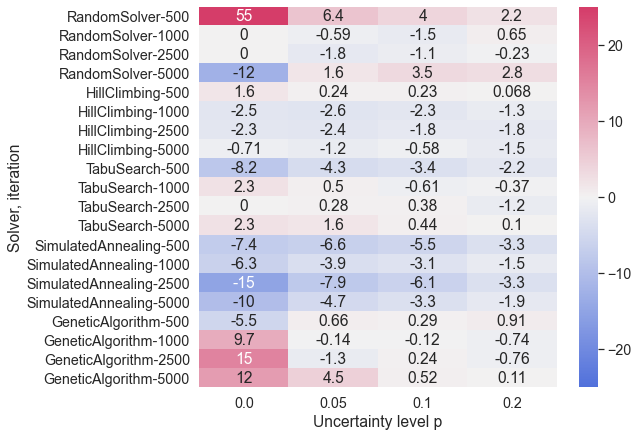
\includegraphics[width=\linewidth]{assets/img/05_Evaluation/heatmap_m1_1.png}
        \caption{Prädiktive gegenüber proaktive Methode}
        \label{fig:evaluation_solver_m1_heatmap_1}
    \end{subfigure}
    \hfill
    \begin{subfigure}{0.497\linewidth}
        \centering
        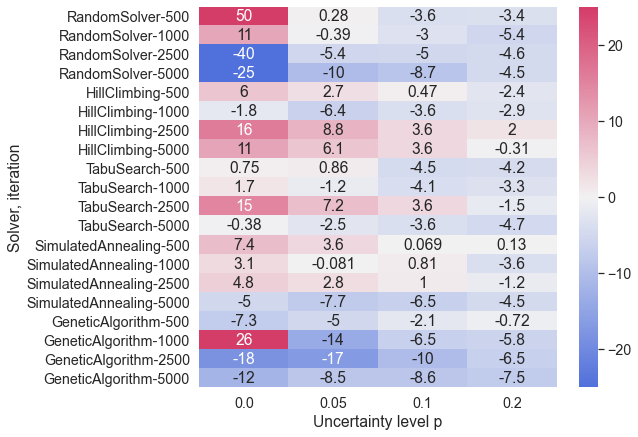
\includegraphics[width=\linewidth]{assets/img/05_Evaluation/heatmap_m1_2.png}
        \caption{Reaktive gegenüber proaktive Methode}
        \label{fig:evaluation_solver_m1_heatmap_2}
    \end{subfigure}
    \par\bigskip 
    \begin{subfigure}{1\linewidth}
        \centering
        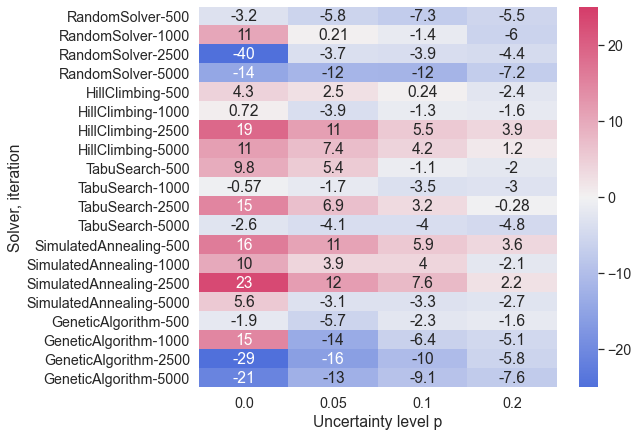
\includegraphics[width=0.5\linewidth]{assets/img/05_Evaluation/heatmap_m1_3.png}
        \caption{Reaktive gegenüber prädiktive Methode}
        \label{fig:evaluation_solver_m1_heatmap_3}
    \end{subfigure}
    
    \caption{Heatmaps der prozentualen Abweichungen für das Instanzset m1}
    \label{fig:evaluation_m1_heatmaps}
    \source{Eigene Darstellungen}
\end{figure}


\begin{figure}[H]

    \begin{subfigure}{0.497\linewidth}
        \centering
        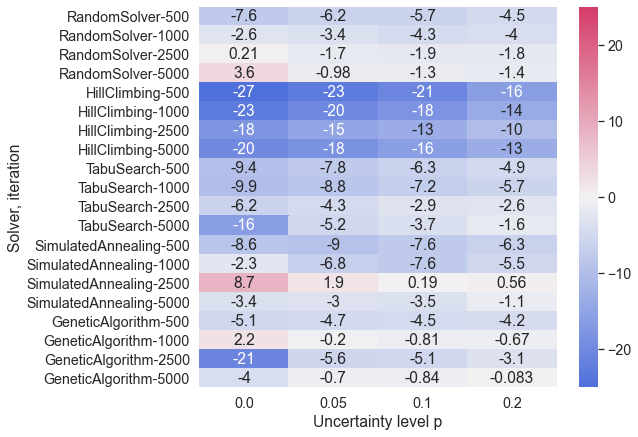
\includegraphics[width=\linewidth]{assets/img/05_Evaluation/heatmap_m2_1.png}
        \caption{Prädiktive gegenüber proaktive Methode}
        \label{fig:evaluation_solver_m2_heatmap_1}
    \end{subfigure}
    \hfill
    \begin{subfigure}{0.497\linewidth}
        \centering
        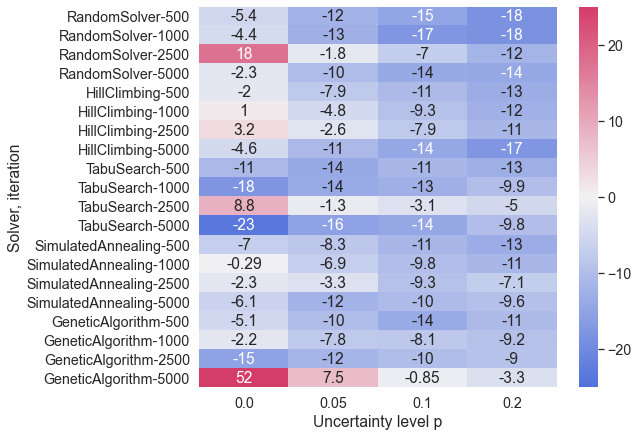
\includegraphics[width=\linewidth]{assets/img/05_Evaluation/heatmap_m2_2.png}
        \caption{Reaktive gegenüber proaktive Methode}
        \label{fig:evaluation_solver_m2_heatmap_2}
    \end{subfigure}
    \par\bigskip 
    \begin{subfigure}{1\linewidth}
        \centering
        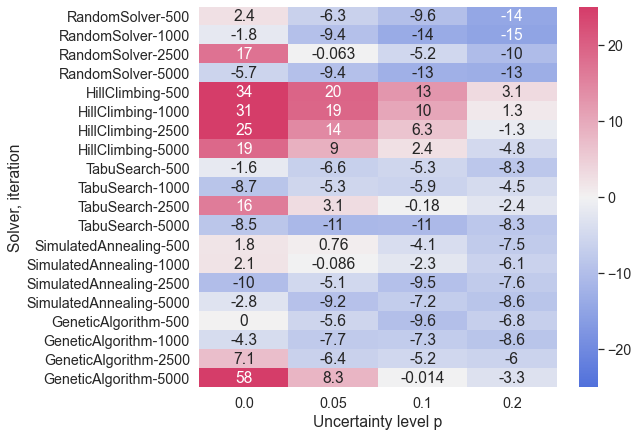
\includegraphics[width=0.5\linewidth]{assets/img/05_Evaluation/heatmap_m2_3.png}
        \caption{Reaktive gegenüber prädiktive Methode}
        \label{fig:evaluation_solver_m2_heatmap_3}
    \end{subfigure}
    
    \caption{Heatmaps der prozentualen Abweichungen für das Instanzset m2}
    \label{fig:evaluation_m2_heatmaps}
    \source{Eigene Darstellungen}
\end{figure}


\begin{figure}[H]

    \begin{subfigure}{0.497\linewidth}
        \centering
        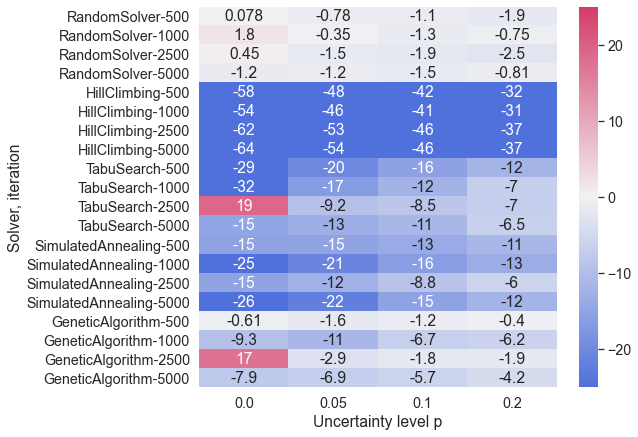
\includegraphics[width=\linewidth]{assets/img/05_Evaluation/heatmap_n0_1.png}
        \caption{Prädiktive gegenüber proaktive Methode}
        \label{fig:evaluation_solver_n0_heatmap_1}
    \end{subfigure}
    \hfill
    \begin{subfigure}{0.497\linewidth}
        \centering
        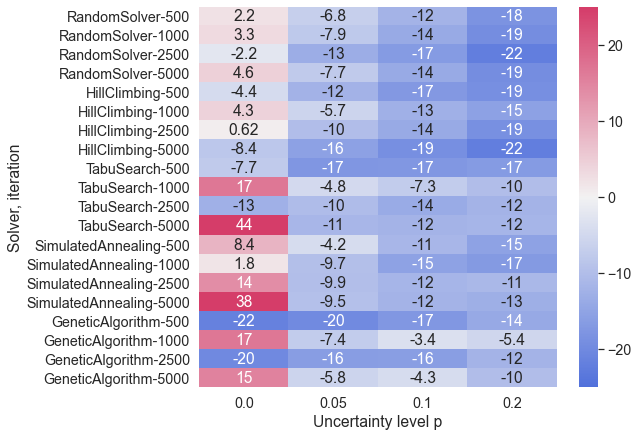
\includegraphics[width=\linewidth]{assets/img/05_Evaluation/heatmap_n0_2.png}
        \caption{Reaktive gegenüber proaktive Methode}
        \label{fig:evaluation_solver_n0_heatmap_2}
    \end{subfigure}
    \par\bigskip 
    \begin{subfigure}{1\linewidth}
        \centering
        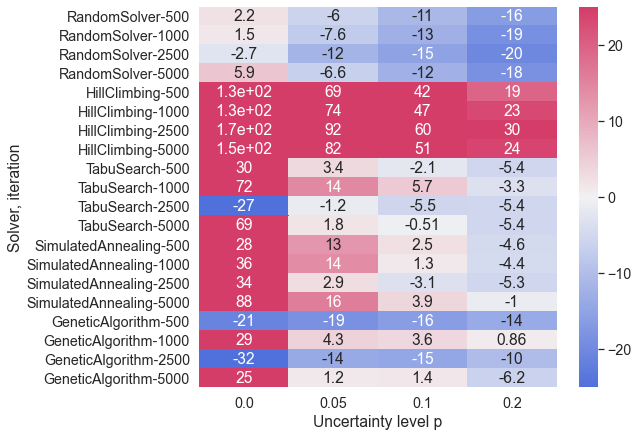
\includegraphics[width=0.5\linewidth]{assets/img/05_Evaluation/heatmap_n0_3.png}
        \caption{Reaktive gegenüber prädiktive Methode}
        \label{fig:evaluation_solver_n0_heatmap_3}
    \end{subfigure}
    
    \caption{Heatmaps der prozentualen Abweichungen für das Instanzset n0}
    \label{fig:evaluation_n0_heatmaps}
    \source{Eigene Darstellungen}
\end{figure}
